\documentclass[a4paper,twoside,11pt,
                %draft,%
              ]{scrbook} 
\usepackage[top=2.5cm,bottom=3.0cm,inner=3.0cm,outer=3.0cm]{geometry}

\usepackage{ifdraft}
\usepackage{ifthen}
\usepackage{amsmath}

%%%%%%%%%%%%%%%%%%%%%%%%%%%%%%%%%%%%%%%%
%\includeonly{abstract,tub-eidesstattliche}
%%%%%%%%%%%%%%%%%%%%%%%%%%%%%%%%%%%%%%%%

%%%% common header file for final and draft mode
\usepackage[utf8]{inputenc}
\usepackage[T1]{fontenc}
%\usepackage{lmodern}
\usepackage[ngerman,UKenglish]{babel}
\usepackage[protrusion, expansion]{microtype}
\usepackage{textcomp}
\usepackage{xspace}
\usepackage[dvipsnames,svgnames]{xcolor}
\usepackage{floatrow}
\DeclareColorBox{imgbg}{\fcolorbox{white}{white}}

\ifdraft{%
    \linespread{1.25}  % Zeilenabstand fuer Korrekturen

\usepackage{geometry}
\geometry{includehead, includefoot, 
    left=30mm,right=25mm, top= 10mm, bottom= 10mm}
\setboolean{@twoside}{false} % einseitiges Layout

\usepackage[missing={Help-missing!}]{gitinfo}

\usepackage{fancyhdr}
\pagestyle{fancy}

%%%% floatrow options
%\floatsetup{capposition=top}
\floatsetup[widefigure]{capposition=bottom,floatwidth=\textwidth}
\floatsetup[table]{capposition=top}

%\usepackage[]{caption}
%\captionsetup{labelfont=bf,font={sf,footnotesize},format=plain,labelsep=period}

\lhead{\rightmark}
\rhead{(\the\day.\the\month.\the\year)~~~-\thepage-}
\lfoot{\footnotesize \emph{Git revision\gitVtags:} \parbox[t]{.60\textwidth}{\gitAuthorIsoDate~\gitReferences}}
\cfoot{}
\rfoot{\footnotesize \emph{Git abbrev. hash}: {\ttfamily\gitAbbrevHash}}
\renewcommand{\footrulewidth}{0.4pt}
\renewcommand{\headrulewidth}{0pt}


}{%
    %%%% Textsatz, Layout, Stil
\usepackage[osf]{mathpazo} % auch Palatino, andere math font
\linespread{1.05}         % Palatino needs more leading (space between lines)
%\usepackage[scaled=0.86]{berasans} % serifenlose Schrift
%\usepackage[scaled]{helvet} serifenlose Schrift
\usepackage[defaultsans]{droidsans} % serifenlose Schrift -- DIE HIER wäre schick!
\usepackage[scaled=1.03]{inconsolata}

%Überschriften serifenlos und über den Rand hängend
\usepackage[sf,sl,outermarks,noindentafter,nobottomtitles]{titlesec}

%könnte alles auch mit \bfseries versehen werden nach Geschmack
\titleformat{\section}[hang]{\LARGE\sffamily}{\thetitle}{8pt}{}
\titleformat{\subsection}[hang]{\Large\sffamily}{\thetitle}{8pt}{}
\titleformat{\subsubsection}[hang]{\large\sffamily}{\thetitle}{8pt}{}
\titleformat{\paragraph}[hang]{\bfseries\sffamily}{\thetitle}{8pt}{}
%Etwas aufwendiger für die Kapitelüberschriften:
\titleformat{\chapter}[display]
{\filleft\Huge\sffamily} %Huge ist die Größe für Titeltext und Nummer
{\fontsize{100pt}{90pt}\selectfont\thechapter}
{-2ex} %is vertical space in [display] mode
%Platz vor dem ganzen Krempel
{\vspace{1ex}}
%Platz danach
[\vspace{1ex}]

%%% TOC design
\usepackage[titles]{tocloft}
\setlength{\cftbeforechapskip}{1ex}
\setlength{\cftbeforesecskip}{0.8ex}
\setlength{\cftbeforesubsecskip}{0.8ex}

%\renewcommand{\cftchapfont}{\sffamily\bfseries}
%\renewcommand{\cftchappagefont}{\sffamily}
%\renewcommand{\cftsecfont}{\sffamily}
%\renewcommand{\cftsecpagefont}{\sffamily}
%\renewcommand{\cftsubsecfont}{\sffamily}
%\renewcommand{\cftsubsecpagefont}{\sffamily}

\renewcommand{\cftpnumalign}{l}
\renewcommand{\cftsecdotsep}{\cftnodots}
\renewcommand{\cftsubsecdotsep}{\cftnodots}
\renewcommand{\cftchapleader}{\hspace{2em}}
\renewcommand{\cftsecleader}{\hspace{2em}}
\renewcommand{\cftsubsecleader}{\hspace{2em}}
\renewcommand{\cftchapafterpnum}{\cftparfillskip}
\renewcommand{\cftsecafterpnum}{\cftparfillskip}
\renewcommand{\cftsubsecafterpnum}{\cftparfillskip}

%%%% Grafiken, Abbildungen
\floatsetup{
    capposition=beside,
    capbesideposition={top,outside},
    facing=yes,
    floatwidth=.75\linewidth,
    capbesidewidth=sidefil,
    capbesidesep=quad,
    floatrowsep=quad,
    %framestyle=colorbox,framearound=all,colorframeset=imgbg,frameset={\fboxrule0pt},
    }
\floatsetup[widefigure]{%
    floatwidth=0.95\textwidth,
    %margins=hangoutside,
    %capposition=beside,
    capposition=below,
    %capbesideposition={top,outside},
    %capbesidewidth=\marginparwidth,
    %capbesideframe=yes,
    %capbesidesep=columnsep,
    %floatrowsep=columnsep,
    %heightadjust=nocaption,
    facing=yes,
    }
\floatsetup[widetable]{%
    floatwidth=0.95\textwidth,
    %margins=hangoutside,
    %capposition=beside,
    capposition=above,
    %capbesideposition={top,outside},
    %capbesidewidth=\marginparwidth,
    %capbesideframe=yes,
    %capbesidesep=columnsep,
    %floatrowsep=columnsep,
    %heightadjust=nocaption,
    facing=yes,
    }
\floatsetup[widefloat]{%
    floatwidth=0.95\textwidth,
    %margins=hangoutside,
    %capposition=beside,
    capposition=below,
    %capbesideposition={top,outside},
    %capbesidewidth=\marginparwidth,
    %capbesideframe=yes,
    %capbesidesep=columnsep,
    %floatrowsep=columnsep,
    %heightadjust=nocaption,
    facing=yes,
    }
\usepackage[]{caption}
\DeclareCaptionLabelSeparator{vbar}{ | } % custom; standard z.B. colon, period, ...
\captionsetup{labelfont=bf,font={sf,footnotesize},format=plain,labelsep=vbar}


}

%%%%% Bibliografie
\usepackage[autostyle,english=british,autopunct]{csquotes}
\usepackage[backend=biber,sorting=nyt,
            %style=authoryear-comp,autocite=footnote,
            style=numeric-comp,autocite=plain,
            firstinits=true,uniquename=init,backref=false,
            maxbibnames=25,minbibnames=10,maxcitenames=2,
            url=false,doi=true,isbn=false,eprint=true,
            ]{biblatex}

\addbibresource{zotero-full.bib}

%%% fine-tuning of the appearance
\AtEveryBibitem{\clearfield{month}}
\AtEveryBibitem{\clearfield{day}}
\renewcommand{\labelnamepunct}{\addcolon\addspace}
\DeclareFieldFormat[article]{volume}{\mkbibbold{#1}}
\DeclareCiteCommand{\citepatent}
    [\mkbibfootnote]
    {\usebibmacro{prenote}}
    {patent \printtext[bibhyperref]{\thefield{number}}}
    {\multicitedelim}
    {\usebibmacro{postnote}}
\DeclareCiteCommand{\supercite}
    [\mkbibsuperscript]
    {%
        \usebibmacro{cite:init}%
        \let\multicitedelim=\supercitedelim
        \iffieldundef{prenote}
        {}
        {\BibliographyWarning{Ignoring prenote argument}}%
        \iffieldundef{postnote}
        {}
        {\BibliographyWarning{Ignoring postnote argument}}%
        \bibopenbracket
    }%
    {\usebibmacro{citeindex}%
    \usebibmacro{cite:comp}}
    {}
    {\usebibmacro{cite:dump}\bibclosebracket}

\DeclareCiteCommand{\mycite}
    []
    {\usebibmacro{prenote}}
    {%
        \printnames[][-\value{listtotal}]{author}: %
        \printfield{title}, %
        \iffieldundef{booktitle}
            {\printfield{journaltitle} }
            {\printfield{booktitle} }
        \printfield{volume}.\printfield{number} (\printfield{year}), %
        \printfield{pages}%
    }
    {\multicitedelim}
    {\usebibmacro{postnote}}

%\DeclareCiteCommand{\publistcite}
    %[]
    %{\usebibmacro{prenote}}
    %{%
        %\printnames[][-\value{listtotal}]{author}: %
        %\printfield{title}, %
        %\printfield{journaltitle} \printfield{volume}.\printfield{number} (\printfield{year}), %
        %\printfield{pages}%
        %\printfield{doi}%
    %}
    %{\multicitedelim}
    %{\usebibmacro{postnote}}

\makeatletter
%%%% use maxbibnames instead of maxcitenames in fullcite:
\DeclareCiteCommand{\fullcite}
  {\defcounter{maxnames}{\blx@maxbibnames}%
    \usebibmacro{prenote}}
  {\usedriver
     {\DeclareNameAlias{sortname}{default}}
     {\thefield{entrytype}}}
  {\multicitedelim}
  {\usebibmacro{postnote}}
\makeatother

\let\cite=\autocite  %% supercite als Standard


%%% nachfolgend Umdefinitionen von Unicode-Zeichen, die
%%% in manchen Zotero-BibLaTeX-Einträgen sind:
\DeclareUnicodeCharacter{00A0}{~}  % non-breaking space
\DeclareUnicodeCharacter{202F}{\,} % narrow non-breaking space
\DeclareUnicodeCharacter{2060}{}   % zero-width space
\DeclareUnicodeCharacter{2002}{\:} % en space
\DeclareUnicodeCharacter{2003}{\;} % em space
\DeclareUnicodeCharacter{2007}{ }  % figure space
\DeclareUnicodeCharacter{2009}{\,} % thin space
\DeclareUnicodeCharacter{2010}{-}  % hyphen
\DeclareUnicodeCharacter{2012}{-}  % figure dash
\DeclareUnicodeCharacter{2013}{--} % en dash
\DeclareUnicodeCharacter{2014}{---}% em dash
\DeclareUnicodeCharacter{2015}{-}  % horizontal bar
\DeclareUnicodeCharacter{2212}{-}  % minus

%%%%% Grafiken, Abbildungen
\usepackage[final]{graphicx} % option final to show images also in draft mode
\usepackage{subfig}
\usepackage{wrapfig}
\usepackage{import}
\usepackage{pgf,tikz}
\usetikzlibrary{positioning}
\usetikzlibrary{patterns}
\usetikzlibrary{intersections}
\usetikzlibrary{shadows}
\usetikzlibrary{spy}
\usetikzlibrary{shapes.symbols, shapes.misc, shapes.geometric, shapes.arrows}
\usetikzlibrary{decorations.markings}
\usepgflibrary{decorations.shapes}
\usetikzlibrary{calc}
\tikzset{>=stealth}


%%%% Tabellen,Listen
\usepackage{tabularx,booktabs,multirow}
\usepackage[inline]{enumitem}
\renewcommand{\labelenumi}{(\roman{enumi})}

%%%% Mathe, Zahlen, chem. Formeln
\usepackage{amsmath,amssymb}
\usepackage{eurosym}
\usepackage{dsfont}
\usepackage[abbreviations=true,
            detect-all,
            product-units = brackets,
            list-units=repeat,
            range-units=repeat,
            multi-part-units=brackets,
            per-mode=reciprocal,
            separate-uncertainty =true,
            range-phrase = \text{ to },
            list-final-separator = \text{ and },
           ]{siunitx}
\DeclareSIUnit{\px}{px}
\DeclareSIUnit[number-unit-product = {\thinspace}]{\inch}{inches}
\DeclareSIUnit{\EUR}{\text{\euro}}

\usepackage[version=3]{mhchem}
\usepackage{xfrac}

%%%% Verschiedenes
\usepackage[para,multiple,stable,perpage,symbol*]{footmisc}
%%% footnote without marker
\newcommand\blfootnote[1]{%
  \begingroup
  \renewcommand\thefootnote{}\footnote{#1}%
  \addtocounter{footnote}{-1}%
  \endgroup
}

%%%% Comment-Sections
\usepackage{comment} %% drinnen lassen fuer Lang-Abstract

%%%% Testen (am Ende entfernen)
%\usepackage{showkeys}
%\renewcommand*{\showkeyslabelformat}[1]{%
%\fbox{\normalfont\tiny\ttfamily#1}}
\usepackage[textsize=scriptsize,bordercolor=none,backgroundcolor=YellowGreen,linecolor=YellowGreen]{todonotes}
%\renewcommand{\todo}[1]{\todo{\sffamily #1}}
\newcommand{\dofig}[1]{\todo[backgroundcolor=DarkSeaGreen,linecolor=none]{\sffamily\textbf{DoFigure:}~#1}\xspace}
\newcommand{\dotxt}[1]{\todo[backgroundcolor=Coral,linecolor=none]{\sffamily\textbf{DoText:}~#1}\xspace}
\newcommand{\doref}[1]{\todo[backgroundcolor=Gold,linecolor=Gold]{\sffamily\textbf{DoRef:}~#1}\xspace}
\newcommand{\doalt}[1]{\textcolor{SkyBlue}{#1}\todo[backgroundcolor=SkyBlue,linecolor=SkyBlue]{\sffamily\textbf{Altrn:}~#1}\xspace}

%%%% Hier kommt's auf die Reihenfolge an
\usepackage{varioref}
\usepackage[pdfpagelabels]{hyperref}
%\usepackage{breakurl} % damit URLs korrekt umgebrochen werden
\usepackage[capitalise]{cleveref}

\ifdraft{%
    \hypersetup{%
            pdftitle={},    
            pdfauthor={Anton Haase},
            pdfcreator={},
            pdfborder=0 0 0,
            breaklinks=true,
            bookmarksopen=true,
            bookmarksnumbered=true,
            linkcolor=black,
            urlcolor=SeaGreen,
            citecolor=SteelBlue,
            colorlinks=true}
}{%
    \hypersetup{%
        pdftitle={},    
        pdfauthor={Anton Haase},
        pdfcreator={},
        pdfborder=0 0 0,
        breaklinks=true,
        bookmarksopen=true,
        bookmarksnumbered=true,
        linkcolor=NavyBlue,
        urlcolor=NavyBlue,
        citecolor=NavyBlue,
        colorlinks=false}

 
%%% Kopf- und Fußzeilen
\newlength{\marginWidth}
\setlength\marginWidth{\marginparwidth+\marginparsep}
\newlength{\fulllinewidth}
\setlength\fulllinewidth{\textwidth+\marginWidth}

\usepackage{truncate} %Um zu lange Kapiteltitel abzuschneiden

\footskip=1.6cm
\makeatletter % = mache @ letter 

%Vordefinition mehrfachverwendeter Teile
\def\oddfootSTANDARD{
   \renewcommand{\@oddfoot}{
       \hbox to\textwidth{\vbox{\hbox to\textwidth{
          \hfill
          \strut
          \hspace{1pt}
       }}}
       \hbox to\marginWidth{\vbox{\hbox to\marginWidth{
          \strut %unsichtbares Zeichen
               \large
               \hspace{5pt}               
               \vrule width 1pt height 1cm
            \hspace{8pt}            
            \textsf{\thepage}
            \hfill
       }}}\hss   
   }
}

\def\evenfootSTANDARD{
   \renewcommand{\@evenfoot}{
      \hspace{-\marginWidth}  
         \hbox to\marginWidth{\vbox{\hbox to\marginWidth{
         \large
         \strut %unsichtbares Zeichen
         \hfill
         \textsf{\thepage}
         \hspace{5pt}
         \vrule width 1pt height 1cm
         \hspace{7pt}
      }}}\hss
   }  
}

%Standardstil für die gesamte Dissertation
\newcommand{\ps@thesis}{%
   \renewcommand{\@oddhead}{%
         \hbox to\textwidth{\vbox{\hbox to\textwidth{%
            \textsf
            \hfill
            \rightmark
            \strut
            \hspace{1pt}
      }}}
         \hbox to\marginWidth{\vbox{\hbox to\marginWidth{%
            \strut %unsichtbares Zeichen
            \hspace{5pt}
            \vrule width 1pt
            \hspace{5pt}
            \textsf
            \thesection
            \hfill
         }}}\hss
   }  
   
   \renewcommand{\@evenhead}{%
      \hspace{-\marginWidth} 
         \hbox to\marginWidth{\vbox{\hbox to\marginWidth{%
            \hfill
            \strut %unsichtbares Zeichen
            \textbf{\textsf{Chapter~\thechapter}}
            \hspace{5pt}
            \vrule width 1pt
            \hspace{7pt}
            \strut
         }}}\hss
         
         \hbox to\textwidth{\vbox{\hbox to\textwidth{%
            \strut %unsichtbares Zeichen
         \truncate{.9\textwidth}{\leftmark}
         \hfill
      }}}\hss
   }
   
   \oddfootSTANDARD   
   \evenfootSTANDARD   
}
%Der PLAIN-Style der Chapter- und Sonderseiten muss redefiniert werden.
\renewcommand{\ps@plain}{%
   \let\@oddhead\@empty
   \let\@evenhead\@empty
   \let\@evenfoot\@empty   
   \oddfootSTANDARD
}
%Spezieller Stil für Inhaltsverzeichnis und Literaturverzeichnis (ohne Nummern wie 0.0 oder B.0)
\newcommand{\ps@thesisINTRO}{%
   \renewcommand{\@oddhead}{%
         \hbox to\textwidth{\vbox{\hbox to\textwidth{%
            \textsf
            \hfill
            \sffamily\rightmark
            \strut
            \hspace{1pt}
         }}}\hss
   } 
   
   \renewcommand{\@evenhead}{%
         \hbox to\textwidth{\vbox{\hbox to\textwidth{%
            \strut %unsichtbares Zeichen
            \truncate{.9\textwidth}{\sffamily\leftmark}
            \hfill
         }}}\hss  
   }
   
   \oddfootSTANDARD   
   \evenfootSTANDARD   
}

%Spezieller Stil für Anhänge
\newcommand{\ps@thesisANHANG}{%
   \renewcommand{\@oddhead}{%
         \hbox to\textwidth{\vbox{\hbox to\textwidth{%
            \textsf
            \hfill
            \rightmark
            \strut
            \hspace{1pt}
         }}}
         \hbox to\marginWidth{\vbox{\hbox to\marginWidth{%
            \strut %unsichtbares Zeichen
            \hspace{5pt}
            \vrule width 1pt
            \hspace{5pt}
            \textsf
            \thechapter
            \hfill
         }}}\hss
   }
   
   \renewcommand{\@evenhead}{%
      \hspace{-\marginWidth}  
         \hbox to\marginWidth{\vbox{\hbox to\marginWidth{%
            \hfill
            \strut %unsichtbares Zeichen
            \textbf{\textsf{Appendix~\thechapter}}
            \hspace{5pt}
            \vrule width 1pt
            \hspace{7pt}
            \strut
         }}}\hss
         
         \hbox to\textwidth{\vbox{\hbox to\textwidth{%
            \strut %unsichtbares Zeichen
            \truncate{.9\textwidth}{\leftmark}
            \hfill
         }}}\hss  
   }
   
   \oddfootSTANDARD
   \evenfootSTANDARD
}


\newcommand{\ps@reallyempty}{%
   \let\@oddhead\@empty
   \let\@evenhead\@empty
   \let\@oddfoot\@empty
   \let\@evenfoot\@empty
}

\renewcommand{\chaptermark}[1]{\markboth{\uppercase{\textsf{#1}}}{}}
\renewcommand{\sectionmark}[1]{\markright{\textsf{#1}}}

\makeatother % = mache @ wieder zu nicht-Buchstaben 
\pagestyle{thesis}


%Problem mit den Seitenzahlen und Headern auf leeren Seiten nach Kapiteln:
\let\origdoublepage\cleardoublepage
\newcommand{\clearemptydoublepage}{%
  \clearpage
  {\pagestyle{empty}\origdoublepage}%
}
\let\cleardoublepage\clearemptydoublepage

}

%%% glossaries for Abbreviations, Glossary
\usepackage[nonumberlist, nomain]{glossaries}
%\usepackage{acronym}
\newglossary[alg]{acronym}{acr}{acn}{\acronymname}
\newglossary[slg]{symbols}{sls}{slo}{\glssymbolsgroupname}
\makeglossaries


%%%%%%%%%%%%%%%%%%%%%%
%%%%% eigene Kommandos
\usepackage{overpic} %for draft text overlays
\usepackage{rotating}
\newcommand{\draftImage}[2]{%
    \begin{overpic}[#1]{#2}
        \put(0,0){\includegraphics[#1]{#2}}
        \put(2,2){\LARGE\color{CornflowerBlue}{\ttfamily\begin{rotate}{45}[Draft]\end{rotate}}}
    \end{overpic}
}
\newcommand{\CD}{\ensuremath{C\mskip-3mu D}\xspace}
\renewcommand{\phi}{\ensuremath{\varphi}\xspace}
\newcommand{\vidx}[2]{\ensuremath{#1_\text{#2}}\xspace}
\newcommand{\eph}{\vidx{E}{ph}}
\newcommand{\ethr}{\vidx{E}{thresh}}
\newcommand{\ali}{\vidx{\alpha}{i}}
\newcommand{\alc}{\vidx{\alpha}{c}}
\newcommand{\alf}{\vidx{\alpha}{f}}
\newcommand{\thf}{\vidx{\theta}{f}}
\newcommand{\dens}{\ensuremath{\varrho}\xspace}
\newcommand{\edens}{\ensuremath{\vidx{\varrho}{e}}\xspace}
\newcommand{\pdepth}{\ensuremath{\Lambda}\xspace}
\newcommand{\ls}{\vidx{L}{s}}
\newcommand{\lpx}{\vidx{L}{px}}
\newcommand{\q}[1]{\vidx{q}{#1}}
\newcommand{\qval}[1]{\ensuremath{\SI[per-mode=reciprocal]{#1}{\per\nm}}\xspace}
\newcommand{\ev}[1]{\ensuremath{\SI{#1}{\eV}}\xspace}
\newcommand{\kev}[1]{\ensuremath{\SI{#1}{\keV}}\xspace}
\newcommand{\qe}{\ensuremath{\mathit{QE}}\xspace}
\newcommand{\nm}[1]{\ensuremath{\SI{#1}{\nm}}\xspace}
\newcommand{\mm}[1]{\ensuremath{\SI{#1}{\mm}}\xspace}
\newcommand{\m}[1]{\ensuremath{\SI{#1}{\m}}\xspace}
\newcommand{\mrad}[1]{\ensuremath{\SI{#1}{\milli\radian}}\xspace}
\newcommand{\mbar}[1]{\ensuremath{\SI{#1}{\milli\bar}}\xspace}

\newcommand{\pvp}{PS-\textit{b}-P2VP\xspace}
\newcommand{\pil}{PILATUS~1M\xspace}
\newcommand{\vpil}{in-vacuum \pil}

\newcommand{\ivec}[2]{\ensuremath{\vidx{\vec{#1}}{#2}}\xspace}
\newcommand{\ivecabs}[2]{\ensuremath{|\ivec{#1}{#2}|}\xspace}
\newcommand{\n}{\ensuremath{\hat{n}}\xspace}
\newcommand{\ft}[1]{\ensuremath{\mathcal{F}(#1)}\xspace}
\newcommand{\dft}[1]{\ensuremath{\mathcal{F}_{\text{DFT}}(#1)}\xspace}
%\newcommand{\psd}[1]{\ensuremath{\mathcal{PSD}(#1)}\xspace}
\newcommand{\psd}[1]{\ensuremath{\mathrm{PSD}(#1)}\xspace}
\newcommand{\hkl}[1]{\ensuremath{\left(#1\right)}\xspace}
\newcommand{\imagu}{\ensuremath{i}\xspace}
\renewcommand{\Re}{\operatorname{\mathfrak{R}}}
\renewcommand{\Im}{\operatorname{\mathfrak{I}}}
\newcommand{\rarr}{\ensuremath{\curvearrowright}\xspace}

\definecolor{data_color}{HTML}{A60628} 
\definecolor{fit_color}{HTML}{348ABD} 


\begin{document}
    \selectlanguage{UKenglish}%
    %%%%% Glossary entries
\newcommand{\newsymentry}[4]{\newglossaryentry{#1}{name=\ensuremath{#2}, description={#3}, sort=#4, type=symbols}}

%% Acronyms
\newacronym{dwba}{DWBA}{distorted-wave Born approximation}
\newacronym{euv}{EUV}{exreme ultraviolet}
\newacronym{xrr}{XRR}{X-ray reflectivity}
\newacronym{eV}{eV}{electron volt}
\newacronym{xrf}{XRF}{X-ray fluorescence}
\newacronym{gixrf}{GIXRF}{grazing incidence X-ray fluorescence}
\newacronym{psd}{PSD}{power spectral density}
\newacronym{rms}{r.m.s.}{root mean square}

%%% Symbols
\newsymentry{dcs}{\ensuremath{\frac{d\sigma}{d\Omega}}}{differential scattering cross section}{sigmaOmega}
\newsymentry{lambda}{\ensuremath{\lambda}}{wavelength}{lambda}
\newsymentry{q}{\ensuremath{\vec{q}}}{\mbox{scattering vector / reciprocal space vector}, ${\vec{q} = \left(\q{x},\q{y},\q{z}\right)^{T}}$}{q}
\newsymentry{k}{\ensuremath{\vec{k}}}{wave vector; the wave number is \mbox{$|\vec{k}| = \gls{k_0} = \sfrac{2\pi}{\gls{lambda}}$}}{k}
\newsymentry{omega}{\ensuremath{\omega}}{frequency}{omega}
\newsymentry{k_0}{\ensuremath{k_0}}{modulus of the wave vector in vacuum (wave number) \mbox{$k_0 = \sfrac{\gls{omega}}{\gls{c}} = \sfrac{2\pi}{\gls{lambda}}$}}{k_0}
\newsymentry{alpha_i}{\ensuremath{\alpha_i}}{angle of incidence defined from the surface normal}{alpha_i}
\newsymentry{alpha_f}{\ensuremath{\alpha_f}}{scattering angle defined from the surface normal}{alpha_f}
\newsymentry{theta_f}{\ensuremath{\theta_f}}{azimutal scattering angle (out-of-plane scattering angle)}{theta_f}
\newsymentry{n}{\ensuremath{n}}{complex index of refraction, $n = \delta + i \beta$}{n}
\newsymentry{epsilon_0}{\ensuremath{\epsilon_0}}{vacuum permittivity or electric constant}{epsilon_0}
\newsymentry{mu_0}{\ensuremath{\mu_0}}{vacuum permeability or magnetic constant}{mu_0}
\newsymentry{c}{\ensuremath{c}}{speed of light in vacuum \mbox{$c = \sfrac{1}{\sqrt{\gls{epsilon_0} \gls{mu_0}}}$}}{c}
\newsymentry{h}{\ensuremath{h}}{Planck's constant, $h=4.135667662(25)\times10^{-15}$ eV$\,$s}{h}
\newsymentry{el_dens}{\ensuremath{\rho_e(\vec{r})}}{electron density at position $\vec{r}$}{rho}
\newsymentry{r_e}{\ensuremath{r_e}}{classical electron radius \mbox{$r_e = \sfrac{e^2}{4 \pi \epsilon_0 m c^2} = 2.82 \times 10^{-5} \AA$}}{r_0}
%% Glossary
%\newglossaryentry{pilatus}{name=PILATUS, description={modular two-dimensional hybrid pixel X-ray detector}}
%\newglossaryentry{ewaldsphere}{name=Ewald sphere, description={construct to visualise the occurrence of scattering spots, the radius is $\sfrac{2\pi}\lambda$}}


\frontmatter

    \pagestyle{thesisINTRO}
    % titlepage.tex

\begin{titlepage}
{\noindent\sffamily\large%
    \begin{center}
        \vspace*{3ex}
        {\LARGE\bfseries\sffamily
            Characterization of Surface and Interface Nanostructures by means of Specular and Diffuse X-ray Scattering
        }
        \vspace{1cm}

        vorgelegt von \\
        Diplom-Physiker \\
        Anton Haase \\
        geboren in Berlin \\
        \vspace{4cm}

        Von der Fakultät II - Mathematik und Naturwissenschaften \\
        der Technischen Universität Berlin \\
        zur Erlangung des akademischen Grades \\
        Doktor der Naturwissenschaften \\
        Dr. rer. nat. \\
        \vspace{3ex}

        genehmigte Dissertation \\
        \vspace{2cm}
    \end{center}

    Promotionsausschuss:
    \vspace{2ex}

    Vorsitzender: Prof. Dr. Mister Unbekannt

    Gutachter: Prof. Dr. Stefan Eisebitt

    Gutachter: Prof. Dr. Mathias Richter

    Gutachterin: Dr. Sa\v{s}a Bajt
    \vspace{1ex}

    Tag der wissenschaftlichen Aussprache:

    \vfill
    \begin{center}
        Berlin 2017
    \end{center}
}
\end{titlepage}

\cleardoublepage


    \section*{Abstract}

\thispagestyle{empty}

    Multilayer mirrors for the \gls{euv} spectral range are essential optical elements of next-generation lithography systems and in scientific applications, e.g.~water window microscopes. Their lack in reaching theoretically predicted peak reflectivity values significantly hinders their applicability and raises the question of the reasons behind that limited performance. This thesis introduces a combination of indirect metrological characterization techniques using EUV and X-ray radiation to enable unambiguous judgments on the structural properties and interface morphologies of those multilayer systems.
    
    The approach was used to study two sets of unpolished and interface polished Mo/Si/C multilayer systems designed to reflect EUV radiation with \nm{13.5} wavelength. They have been fabricated with increasing molybdenum thickness from sample to sample. By examining the combination of \gls{euv} reflectivity and \gls{xrr} and considering experimental uncertainties, structural parameters could be reconstructed and validated by deducting confidence intervals. By establishing a method for the analysis of \gls{euv} diffuse scattering, an observed minimum in the peak reflectance for some samples could be related to variations in layer thickness and interface roughness associated with crystallization in the molybdenum layers. Increased roughness for samples at the crystallization threshold and intermixing could be identified impeding the measured reflectance.
    
    Furthermore, this methodology was applied to Cr/Sc multilayer mirrors for the water window spectral range having individual layer thicknesses in the sub-nanometer regime. The combination of the analysis of \gls{euv} reflectivity and of \gls{xrr} based on a binary layer model was shown to be insufficient to describe this system. The model was extended to explicitly take into account gradual interface profiles and strong intermixing. It was demonstrated by structural characterization and systematic validation of the extended model parameters, based on the analysis of \gls{euv} reflectivity, \gls{reuv}, \gls{xrr} and \gls{xrf} experiments, that only the combination of those analytic methods yields a consistent result. By augmenting the characterization through the \gls{euv} diffuse scattering analysis, the cause for the low reflectivity was determined.

\cleardoublepage

\thispagestyle{empty}
\selectlanguage{ngerman}

\section*{Zusammenfassung}
    
    Mehrschichtspiegel für den \gls{euv} Wellenlängenbereich sind wichtige optische Komponenten für die nächste Halbleiterlithografiegeneration und kommen auch im wissenschaftlichen Bereich beispielsweise in Mikroskopen für das Wasserfenster zum Einsatz . Deren verminderte Reflektivität im Vergleich zu den theoretisch möglichen Werten schränkt ihre Einsatzfähigkeit ein und wirft die Frage nach den Ursachen dafür auf. In der vorliegenden Dissertation wurde eine Kombination von metrologischen indirekten Charakterisierungstechniken unter Anwendung von EUV und Röntgenstrahlung eingeführt. So wurden Rückschlüsse auf die Struktur und Grenzflächenmorphologie der Mehrschichtsysteme eindeutig möglich.
    
    Die Methodik wurde zur Untersuchung von Mo/Si/C-Mehrschichtsystemen mit polierten und unpolierten Grenzflächen eingesetzt, welche als Spiegel für EUV-Strahlung mit \nm{13.5} Wellenlänge dienen. Die Mehrschichtsysteme waren mit wachsender Molybdänschichtdicke von Probe zu Probe hergestellt. Die kombinierte Analyse von \gls{euv}-Reflektivität und Röntgenreflektivität unter Berücksichtigung der experimentellen Unsicherheiten ermöglichte eine Bestimmung der strukturellen Modellparameter und deren Konfidenzintervalle. Die Einführung einer Methode zur Analyse diffuser \gls{euv} Streuung erlaubt ferner die Korrelation beobachteter Reflektivitätseinbrüche in bestimmten Proben mit Variationen der Schichtdicken und der Grenzflächenrauigkeit durch Kristallisation in den Molybdänschichten. Erhöhte Rauigkeit an der Kristallisationsschwelle und Durchmischung an den Grenzflächen konnten als Ursache der beinträchtigten Reflektivität eindeutig identifiziert werden.
	
    Die hier etablierte Methodologie wurde desweiteren auf Cr/Sc-Mehrschichtspiegel für das Wasserfenster angewandt. Die Kombination von \gls{euv}- und Röntgenreflektivität basierend auf einem binären Schichtmodell stellte sich bei diesem System als unzureichende Beschreibung heraus. Daher wurde das Modell erweitert, um graduelle Grenzflächenprofile und starke Vermischung explizit zu berücksichtigen. Auf Grundlage der Strukturanalyse mittels \gls{euv}-Refklektivität, resonanter \gls{euv}-Reflektivität, Röntgenreflektivität und Röntgenfluoreszenz und anschließender Validierung kontte gezeigt werden, dass nur die Kombination all dieser analytischen Methoden ein konsistentes Ergebnis liefert. Die Erweiterung dieser Charakterisierung durch diffuse \gls{euv}-Streuung erklärt eindeutig die Ursachen für die geringe Reflektivität.

\selectlanguage{UKenglish}
\cleardoublepage



    \selectlanguage{UKenglish}%
    \tableofcontents
    \listoffigures
    \listoftables

    %\ifdraft{%
        %% titlepage.tex

\begin{titlepage}
\begin{center}

    \vspace*{0.2\paperheight}

    \rule{\linewidth}{0.5mm} \\[0.4cm]
    {\huge\bfseries\sffamily When size does matter:} \\[1ex]
    {\LARGE\sffamily Dimensional metrology of nanostructured layers and surfaces using X-rays} \\
    \rule{\linewidth}{0.5mm} \\[4cm]


    {\sffamily%
    vorgelegt von \\Diplom-Physiker Jan Wernecke \\zur Erlangung des akademischen Grades \\Doktor der Naturwissenschaften (Dr. rer. nat.).}

    \vfill
    {%
    \sffamily%
    \begin{otherlanguage}{ngerman}
        Berlin, \today
    \end{otherlanguage}
    }
\end{center}
\end{titlepage}


        %\newpage
        %\thispagestyle{empty}
        %\mbox{}

        %\tableofcontents
        %\addtocontents{toc}{\protect\thispagestyle{fancy}}
    %}{%
        %\pagestyle{thesisINTRO}
        %\tableofcontents
    %}

    \printglossary[type=\acronymtype,title=Abbreviations,style=list]
    \printglossary[type=symbols,title=Symbols,style=long,nonumberlist=true]

\mainmatter
    \ifdraft{}{\pagestyle{thesisINTRO}}
    %\include{pIntro}
    \ifdraft{}{\pagestyle{thesis}}
    \chapter{Mo/Si Multilayer}

\section{Introduction} Multilayer systems have been of great interest over the past decades. The first applications of multilayers serving as mirrors for soft X-rays were optical components for space probes. The main driving force today is the shift in direction towards the EUV spectral range at 13.5 nm wavelength in optical lithography for the semiconductor industry. Lenses in classic lithography systems are replaced by multilayer mirrors. High  reflectivities are achieved by utilizing the constructive interference of the reflected light at each interface when fulfilling the Bragg condition. State of the art Mo/Si multilayer mirrors reach reflectivities of up to 70\% \cite{braun2002mo, Feigl2006703} in the case of near-normal incidence EUV radiation. This value is still well below the theoretical limit of approx.~75\% for an ideal multilayer. An important reason for the loss of reflectivity is interface imperfections such as roughness and interdiffusion causing diffuse scattering. The analysis of the off-
specular scattering 
thus serves as a 
natural tool for the characterization of interfacial roughness. 

At the Physikalisch-Technische Bundesanstalt (PTB), angle and energy resolved scatterometric measurements have been performed to analyze the off-specular scattering using EUV radiation. The tunability of synchrotron radiation in conjunction with angular resolution allows obtaining two-dimensional intensity maps close to the relevant multilayer resonance for near-normal incidence geometries. The diffuse scattering from interface roughness contains information on its morphology, such as lateral and vertical correlations, its jaggedness, and mean amplitude. A rigorous analysis of the reciprocal space represented through the scattering pattern, thus, provides access to the interface morphology.

Scatterometry poses an inverse problem of gaining information about the properties of the interfaces. A theoretical model of the diffuse scattering is required to yield a reconstruction of the actual sample and deduct the power spectral density (PSD) of roughness. The topic of experimental and theoretical analysis towards the characterization of roughness involving optical wavelengths has been largely studied by others and published in the optical community \cite{Amra:93_2,Amra:94, Elson:80, Elson:83, Schroder:11, Schroder:14}. We take a different approach involving the analysis of diffuse EUV scattering employing numerical simulations of the expected scattering distribution based on the distorted-wave Born approximation (DWBA)~\cite{PhysRevB.49.10668,PhysRevB.47.15896}.

We will show that a rigorous, dynamic calculation of the EUV radiation interacting with the multilayer is required to obtain the power spectral densities. The influence of multiple reflections at the layer boundaries cannot be neglected in this analysis. The simulations are compared to measured data obtained for high-reflectance Mo/Si multilayers. The influence of the measurement geometry of the diffuse scattering is discussed in detail.

\section{Experimental Methods} \label{sec:experimental} The experiments were conducted at the soft X-ray radiometry beamline of the PTB laboratory \cite{Beckhoff2009}. It is located at the electron storage ring for synchrotron radiation BESSY II in Berlin-Adlershof. The beamline offers a tunable spectral range from $0.7$ nm to $35$ nm in combination with a highly collimated photon beam \cite{ptbbeamline}. The total collimation at the experimental station is below $200\,\mu\text{rad}$, while the scatter halo of the beam is suppressed to below $10^{-5}$ relative intensity within $1.7$ mrad with respect to the center of the beam.

The measurements were performed using angle and energy resolved scatterometry. The experimental station is contained in a vacuum chamber allowing measurements at pressures below $10^{-7}$ mbar. The sample holder is placed on a goniometer \cite{PTBBigRef}. The scatter intensities presented in this study were recorded in the reflection plane using a GaAsP photodiode. This setup offers a wide angular range for specular and off-specular measurements. 

The sample used in the experiments is a high-reflectance multilayer with $68.5(7)$ \% reflectivity at an angle of incidence of $\alpha_i = 6.75^\circ$ and a wavelength of $13.5$ nm. The silicon substrate was coated with a multilayer stack of molybdenum (Mo) and silicon (Si) with B$_4$C and carbon interdiffusion layers with a number of periods of 65. It was fabricated using magnetron sputtering at the Frauenhofer IWS, Dresden \cite{braun2002mo}. To determine the composition of the multilayer, the reflectivity was measured in a wavelength range of $10$ nm to $16$ nm. 

In order to gain information on interfacial roughness, the off-specular scattering of the multilayer sample was measured in different geometries. We performed coplanar rocking and detector scans as shown in Fig.~\ref{fig:measurementGeometry}.
\begin{figure}
        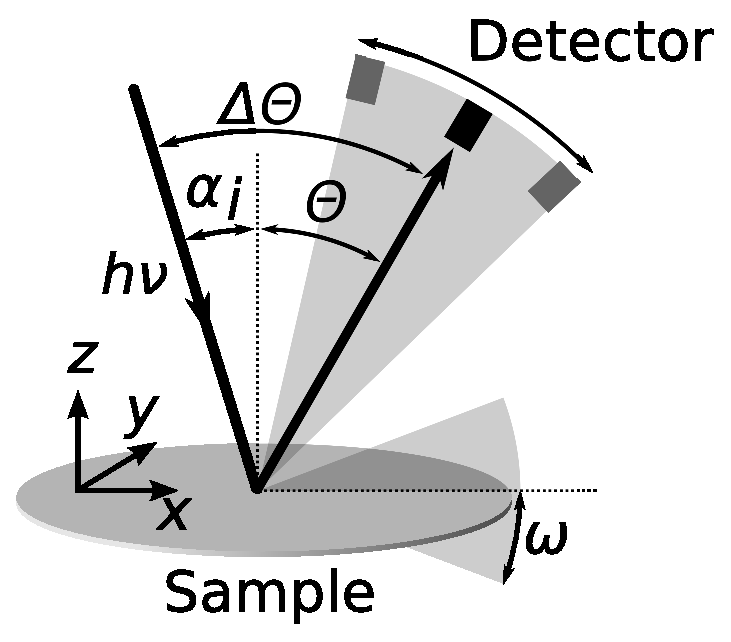
\includegraphics[width=0.3
        \textwidth]{img/im_mo_si/Streugeometrie} \caption{Co-planar measurement geometries. By keeping the opening angle $\Delta\Theta$ between incident and exit beam and the detector fixed, respectively, a rocking scan can be performed by changing the sample angle $\omega$. In a detector scan the sample angle $\omega$ is kept fixed and defines the angle of incidence while the detector is moved along $\Theta$.} \label{fig:measurementGeometry} 
\end{figure}
\begin{figure}
        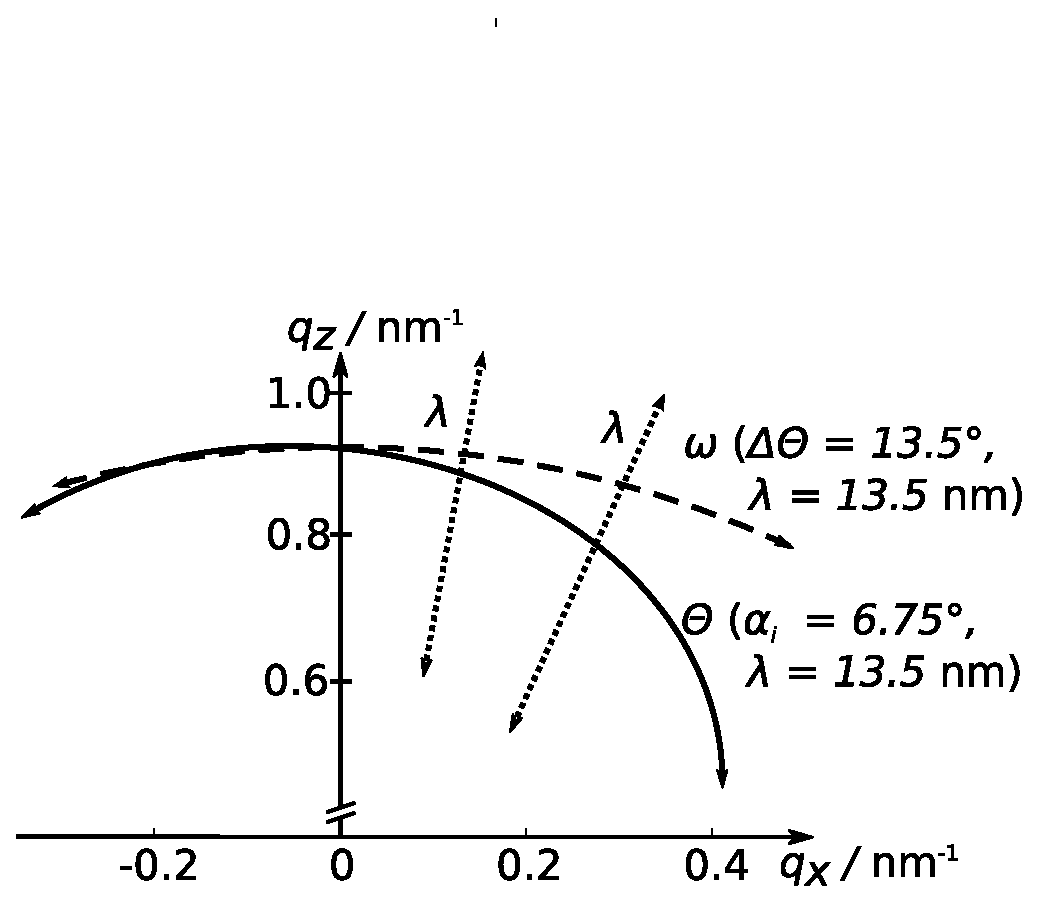
\includegraphics[width=0.45
        \textwidth]{img/im_mo_si/Qspace_paths} \caption{Schematic positions in reciprocal space in dependence on the measurement geometry. The dashed path represents a rocking scan with the angle $\omega$. The solid line shows the movement in $q$-space when changing the detector angle $\Theta$ at a fixed angle of incidence. By tuning the wavelength at each angular position, the $q_z$-direction becomes accessible as indicated by the dotted arrows.} \label{fig:pathsInQ} 
\end{figure}
The corresponding paths through reciprocal space are different for these two cases. They are shown schematically in Fig.~\ref{fig:pathsInQ}. In addition, a wavelength scan ($\lambda$-scan) was performed at each angular position. By changing the wavelength and the angle in the same measurement, both degrees of freedom ($q_x$ and $q_z$) in reciprocal space become accessible. Following this method, we recorded two-dimensional reciprocal space maps of the vicinity of the first Bragg resonance. The reciprocal space coordinates in terms of the experimental parameters are given by 
\begin{align}
        q_x &= \frac{2 \pi}{\lambda} \big(\sin(\Theta) - \sin(\alpha_i)\big) \text{,}\\
        q_z &= \frac{2\pi}{\lambda} \big(\cos(\Theta) + \cos(\alpha_i)\big) \text{,} 
\end{align}
where $\lambda$ is the wavelength of the incoming light, $\Theta$ is the exit angle with respect to the surface normal (detector angle) and $\alpha_i$ is the angle of incidence with respect to the surface normal.

\begin{figure*}
        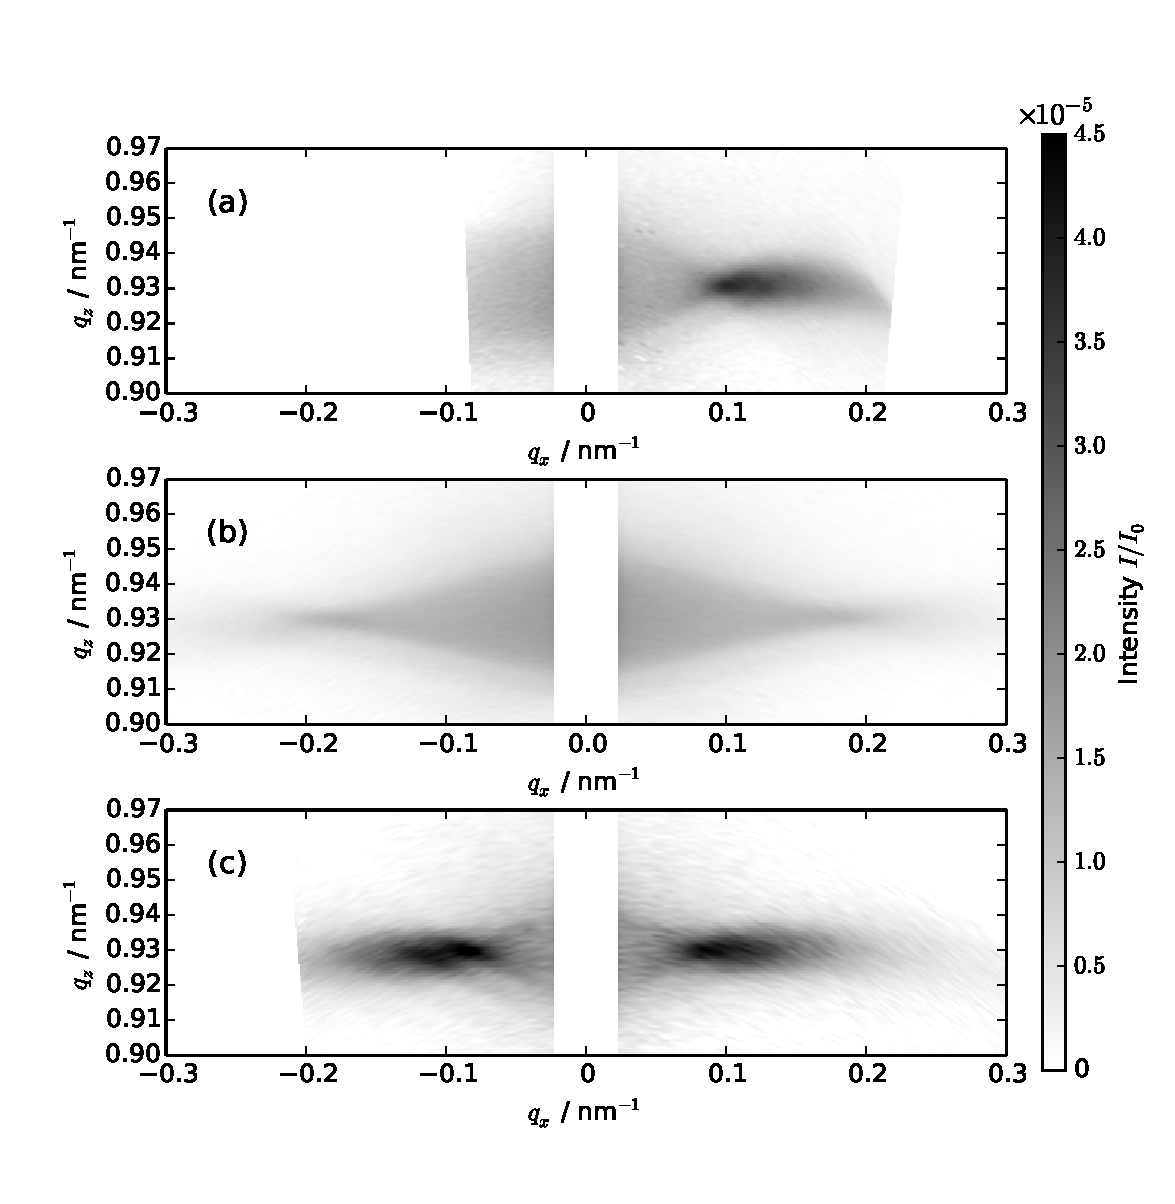
\includegraphics[width=
        0.8\textwidth]{img/im_mo_si/measured_maps} \caption{Measured intensity map of a detector scan of a Mo/Si multilayer mirror at an angle of incidence $\alpha_i = 6.75^\circ$ (a) and  measured intensity maps of the identical sample obtained through rocking scans at an opening angle between detector and incident beam of $\Delta \Theta = 13.5^\circ$ (b) and $\Delta \Theta = 30^\circ$ (c). The area close to the specular axis was excluded from this dataset due to its strong intensity compared to the diffuse scattering shown here. The access to the negative $q_x$-axis in (a) is limited due clipping of the incoming beam with the detector.} \label{fig:comparison} 
\end{figure*}
\subsection{Reciprocal Space Maps for Different Measurement Geometries} The reciprocal space maps in Fig.~\ref{fig:comparison} for the rocking scan (b) at an opening angle of $\Delta \Theta = 13.5^\circ$ and the rocking scan (c) at an opening angle of $\Delta \Theta = 30^\circ$ (corresponding to an angle of incidence of $\alpha_i = 6.75^\circ$ and $\alpha_i = 15.0^\circ$, respectively, in specular geometry) and for the detector scan with the angle of incidence $\alpha_i = 6.75^\circ$ clearly show different symmetries. We observe a strong enhancement in the off-specular scattering around $q_x\approx0.1$ nm$^{-1}$ (cf.~Fig.~\ref{fig:comparison}(a) and Fig.~\ref{fig:comparison}(c)), which is not replicated on the negative $q_x$-axis in case of (a). The rocking scans \ref{fig:comparison}(b) and \ref{fig:comparison}(c) are symmetric with respect to the specular axis at $q_x=0$, however, no enhanced scattering appears in (b). The latter map shows a triangular-shaped intensity distribution for both the positive and 
negative $q_x$ range. A minimum in width with respect to the $q_z$ direction can be observed here around $q_x \approx \pm 0.2$ nm$^{-1}$. The triangular shape also appears for the 
positive $q_x$ range 
of the detector scan in Fig.~\ref{fig:comparison}(a), where the minimum in width coincides with the intensity maximum.


In Fig.~\ref{fig:BraggSheet_DetectorAndRocking}, the three measurements shown above are compared by considering the intensity distribution along $q_z=0.93$ nm$^{-1}$, which corresponds to the momentum transfer at the multilayer resonance. The differences in the off-specular scattering are evident. 
\begin{figure}
        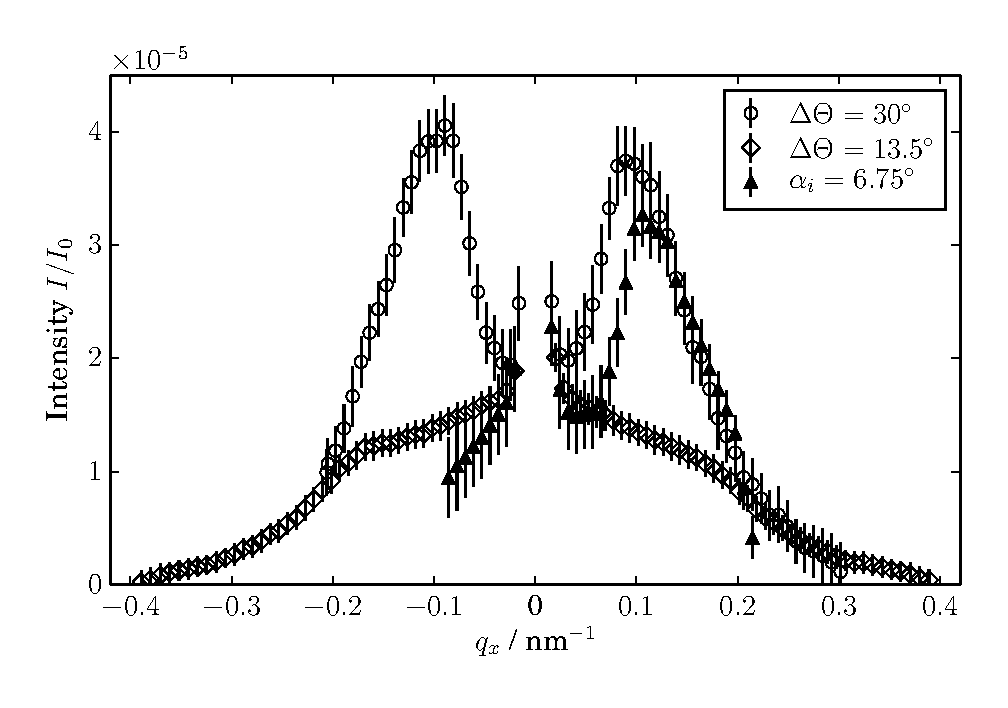
\includegraphics[width=0.5
        \textwidth]{img/im_mo_si/BraggSheet_DetectorAndRocking} \caption{Averaged diffuse scattering intensity along $q_x$ in the interval  $q_z=(0.930 \pm 0.003$) nm$^{-1}$ corresponding to the resonance of the multilayer. The data shown are two rocking scan and one detector scan geometries (see text for details).} \label{fig:BraggSheet_DetectorAndRocking} 
\end{figure}

The measurement geometry dependence of the reciprocal space maps indicates that the intensity distributions cannot be the result of multilayer roughness properties alone, i.e. the power spectral density. Scattering intensities caused by roughness occur at identical positions in reciprocal space for any measurement geometry. In order to explain the observations shown here, the proper theoretical description of the diffuse scattering distributions is presented in the following section.

\section{Theoretical Background} \label{sec:theory} Our theoretical description of the diffuse EUV scattering from multilayers is based on the distorted-wave Born approximation (DWBA)~\cite{PhysRevB.49.10668,PhysRevB.47.15896}, widely used in the analysis of hard X-ray scattering. The DWBA is a perturbation theory in which the interfacial roughness is considered to be a small deviation from the ideal multilayer. This corresponds to a potential in the wave equation 
\begin{equation}
        (\Delta + K^2) |E(\mathbf{r})\rangle = V(\mathbf{r}) |E(\mathbf{r})\rangle\text{,} \label{eqn:wave_equation} 
\end{equation}
of $V(\mathbf{r}) = V_\text{id}(\mathbf{r}) + V_\text{r}(\mathbf{r})$ that can be separated into a strong part $V_\text{id}(\mathbf{r})$ for which an analytical solution exists and a small perturbation $V_\text{r}(\mathbf{r})$ describing the interfacial roughness. In case of a multilayer, we start from the dynamic calculation of the electric fields of a perfectly flat multilayer. The wave equation Eq.~\eqref{eqn:wave_equation} is solved by calculating the field amplitudes using a matrix formalism \cite{PrinciplesOfOptics}.

For the calculation of the specular reflectivity curve it is necessary to correct the field calculation for the interfacial roughness and diffusion. Modified Fresnel coefficients according to N\'evot/Croece \cite{nevot_croece} assuming a Gaussian interface profile are used, 
\begin{align}
        r^{(j)} &= r_{id}^{(j)} \exp(-2 k_z^{(j)} k_z^{(j+1)} \sigma_j^2)\text{,} \label{eqn:fresnel_r}\\
        t^{(j)} &= t_{id}^{(j)} \exp((k_z^{(j)} - k_z^{(j+1)})^2 \sigma_j^2/2) \text{,} \label{eqn:fresnel_t}
\end{align}
where $r_{id}^{(j)}$ and $t_{id}^{(j)}$ are the Fresnel reflection and transmission coefficients, respectively, for the ideal  $j^\text{th}$ interface, $\sigma_j$ is the root mean square roughness (rms) and $k_z^{(j)}$ is the $z$-component of the incidence wave vector at the $j^\text{th}$ interface.

The diffuse scattering cross section is given by the covariance of the matrix element of the perturbation potential on the basis of the wave functions from the analytic solution for a given incidence and exit angle \cite{PhysRevB.38.2297,PhysRevB.49.10668} 
\begin{equation}
        \underset{\text{diffuse}}{\Big(\frac{d \sigma}{d \Omega}\Big)}= \text{Cov}(\langle E_{\text{id},1}| V_r|E_{\text{id},2}\rangle)\text{,} \label{eqn:incoherent_cross_section} 
\end{equation}
where $|E_{\text{id},i}\rangle\text{, }i =1,2$ are the solutions of the wave equation Eq.~\eqref{eqn:wave_equation} for the ideal multilayer and the given incidence and exit angles, respectively, calculated using the unmodified Fresnel coefficients $r_{id}^{(j)}$ and $t_{id}^{(j)}$ representing the perfectly flat multilayer. Since the roughness potential is non-zero only at the individual interfaces, Eq.~\eqref{eqn:incoherent_cross_section} can be decomposed into a sum over the matrix elements at each interface $j$. In the following, we use the small roughness $q_{z,j} \sigma_j \ll 1$ approximation which is valid for any high-quality multilayer mirror (cf. \cite{PhysRevB.53.6048} for the more general expression).

In the case of small reflectivity amplitudes, dynamic multiple reflections are often neglected and the dominant term in the decomposition is diffuse scattering of the transmitted fields at the roughness of each interface. The so-called semi-kinematic approximation \cite{PhysRevB.38.2297} yields an explicit expression for Eq.~\eqref{eqn:incoherent_cross_section} with
\begin{align}
                \overset{\text{semi-kinematic}}{\underset{\text{diffuse}}{\Big(\frac{d \sigma}{d \Omega}\Big)}} = &\frac{A \pi^2}{\lambda^4}\sum \limits_{j=1}^{N}\sum \limits_{i=1}^{N} \Big((n_j^2 - n_{j+1}^2)^* (n_i^2 - n_{i+1}^2) \nonumber \\ &\qquad\times T^{(1)*}_j T^{(2)*}_j T^{(1)}_i T^{(2)}_i S_{i j}(q_x)\Big)\text{,} \label{eqn:semi_kinematic_theory} 
\end{align}
where $A$ is the illuminated sample area, $\lambda$ the wavelength of the incident light and $n_j$ is the complex index of refraction of material $j$. The $T^{(1,2)}_j$ are defined as the amplitude of the transmitted field at the interface $j$ for the given exit angle (2) (represented as a time-inverted beam originating at the detector) and incidence angle (1). The total field at the $j$th interface is expressed in terms of the reflected field $E_r^{(j)}(z)$ propagating towards the vacuum and the transmitted field $E_t^{(j)}(z)$ propagating towards the substrate
\begin{align}
        E_t^{(j)}(z) &= T_{j} e^{i k_z^{(j)} z} \text{,} \\
        E_r^{(j)}(z) &= R_{j} e^{-i k_z^{(j)} z} \text{,} 
\end{align}
with $E_{id}^{(j)}(\mathbf{r}) = e^{i \mathbf{k_\parallel r_\parallel}} (E_t^{(j)}(z) + E_r^{(j)}(z))$ being the full solution of the wave equation Eq.~\eqref{eqn:wave_equation} for the ideal multilayer at the $j^\text{th}$ interface. $S_{ij}(q_x)$ is the structure factor describing the influence of the interfacial roughness on the diffuse scattering intensity defined through
\begin{widetext}
\begin{align}
S_{ij}(\vec{q}_\parallel; q_z^{(j)}, q_z^{(i)}) = &\frac{\exp \Big[-((q_z^{(j)*})^{2} \sigma_j^2 + (q_z^{(i)})^{2} \sigma_i^2)/2\Big]}{q_z^{(j)*} q_z^{(i)}} \int d^2 \vec{X} \Big(\exp [q_z^{(j)*} q_z^{(i)} C_{ij}(\vec{X})]-1\Big) \exp(i \vec{q}_\parallel \cdot \vec{X}) \text{,} \label{eqn:full_structure_factor}
\end{align}
\end{widetext}
where $q_z^{(i)}$ is the $z$-component of the scattering vector $\vec{q}$ at the $i$th interface, $\vec{X} = \vec{x} - \vec{x}'$ is the lateral distance vector and $C_{ij}(\vec{x}-\vec{x}') = \langle h_i(\vec{x}) h_j(\vec{x}') \rangle$ is the correlation function of the interface profiles $h(\vec{x})$ of the interfaces $i$ and $j$ \cite{PhysRevB.51.5297,PhysRevB.53.6048}. In case of the small roughness approximation, \begin{align}
\frac{\exp \Big[-((q_z^{(j)*})^2 \sigma_j^2 + (q_z^{(i)})^{2} \sigma_i^2)/2\Big]}{q_z^{(j)*} q_z^{(i)}} \approx \frac{1}{q_z^{(j)*} q_z^{(i)}}
\end{align}
and $\exp [q_z^{(j)*} q_z^{(i)} C_{ij}(\vec{X})]-1 \approx q_z^{(j)*} q_z^{(i)} C_{ij}(\vec{X})$ apply and Eq.~\eqref{eqn:full_structure_factor} reduces to
\begin{align}
S_{ij}(\vec{q}_\parallel) \approx \int d^2 \vec{X} C_{ij}(\vec{X}) \exp(i \vec{q}_\parallel \cdot \vec{X}) \text{.} \label{eqn:reduced_structure_factor}
\end{align}
$S_{ij}(\vec{q}_\parallel)$ is, thus, the Fourier transform of the correlation function $C_{ij}(\vec{X})$. In case of co-planar scattering furthermore $\vec{q}_\parallel \equiv \vec{q}_x$.
Assuming identical growth for the individual layers, i.e.~a material independent propagation of roughness along the $z$-direction, $S_{ij}(q_x)$ can be expressed in terms of the lateral power spectral density (PSD) $C_{i}(q_x)$ and a vertical replication factor $c_{ij}^{\perp}(q_x)$ \cite{spiller1993multilayer},
\begin{equation}
        S_{ij}(q_x) = c_{ij}^{\perp}(q_x) C_{\text{max}(i,j)}(q_x)\text{.} \label{eqn:factorized_structure_factor}
\end{equation}

Other PSD functions based on different models of lateral interface roughness correlation have been proposed, e.g.~by Sinha et al.~\cite{PhysRevB.38.2297}. We follow the approach by de Boehr et al.~\cite{deBoerLateralCorrelation,PhysRevB.51.5297} for fractal interface roughness, where the lateral correlation function of the $i$th interface is given by
\begin{align}
\tilde{C}_i(\vec{X}) = P_i \xi_\parallel^{H_i} |\vec{X}|^{H_i} K_{H_i}\Big(|\vec{X}|/\xi_\parallel\Big) \text{.} \label{eqn:lateral_correlation_function}
\end{align}
$H_i$ is the Hurst factor providing a measure for the jaggedness of the interface \cite{PhysRevB.38.2297}, $K_{H_i}$ are the modified Bessel functions of the order $H_i$, $\xi_\parallel$ is a lateral correlation length and
\begin{align}
P_i = \frac{\sigma_i^2}{\xi_\parallel^{H_i-1} 2^{H_i-1} \Gamma(1+H_i)/H_i}\text{.}
\end{align}

Our goal is to determine a single average power spectral density. We thus do not distinguish between individual interfaces in the model and assume an identical roughness properties for all interfaces. Hence $\sigma_j = \sigma$, $H_j = H$ and $C_{\text{max}(i,j)}(q_x) = C(q_x)$. The PSD is given by the Fourier transform of Eq.~\eqref{eqn:lateral_correlation_function} with respect to $q_x$, which yields the closed analytic form
\begin{equation}
        C(q_x) = \frac{4 \pi H \sigma^2 \xi_\parallel^2}{(1+|q_x|^2\xi_\parallel^2)^{1+H}} \text{.} \label{eqn:psd} 
\end{equation}


The high degree of thickness stability for well-defined multilayers as is necessary for high-performance mirrors implies a high degree of vertical correlation of individual interfaces roughness throughout the stack. In order to derive the replication factor in Eq.~\eqref{eqn:factorized_structure_factor}, we follow Stearns et al.~\cite{stearns:4286}. In this model, the evolution of the surface roughness $w(x,y)$ during the growth of a single layer is described by the Langevin equation. In its Fourier transformed form, 
\begin{align}
\frac{\partial w(f)}{\partial t} = - 4 \pi^2 v f^2 w(f) + \frac{\partial \eta(f)}{\partial t} \text{,} \label{eqn:langevin}
\end{align}
where $v$ is a diffusion-like parameter, $\eta(f)$ is random noise normalized to the layer thickness and $w(f)$ describes the roughness evolution in dependence of the spacial frequency $f$. The roughness evolution during the growth of a single layer of a specific material can then be evaluated by discritizing Eq.~\eqref{eqn:langevin} for the successive deposition of material of thickness $\delta d$
\begin{align}
w_i(f) = c_\perp(f;\delta d) w_{i-1}(f) + \eta(f) \text{,}
\end{align}
where $c_\perp(f;\delta d)$ is the replication factor of roughness for a single deposition. In the limit of repeated infinitesimal depositions until the full $n$th layer of thickness $d_n$ is grown, $c_\perp(f,d_n)$ can be evaluated to be \cite{spiller1993multilayer}
\begin{align}
    c_\perp(f,d_n) &= \exp(-4\pi^2 f^2 v \,d_n) \nonumber \\
                   &= \exp(-q_x^2 v \,d_n)\text{,}
\end{align}
with $q_x^2 = 4 \pi^2 f^2$. Assuming identical diffusionlike behavior $v$ for all materials of a multilayer and defining $\xi_\perp(q_x) = 1/(v q_x^2)$, the replication factor in Eq.~\eqref{eqn:factorized_structure_factor} is given by
\begin{align}
c_{ij}^\perp(q_x) =  \exp\Bigg(-\sum \limits_{n = \text{min}(i,j)}^{\text{max}(i,j)-1}d_n/\xi_\perp(q_x) \Bigg)\text{.}
\end{align}
Here, $\xi_\perp(q_x)$ can be interpreted as a frequency dependent vertical correlation length, describing the distance perpendicular to the stack until the replication factor decreased to $1/e$.

Gullikson et al.~\cite{PhysRevB.59.13273} observed that the direction of the vertical replication of roughness can be tilted with respect to the surface normal. This leads to tilted Bragg planes requiring a coordinate transformation in reciprocal space to account for the tilt angle $\beta$ according to
\begin{align}
\overline{q}_z = q_z - q_x \tan \beta\text{.}
\end{align}
Since the vertical scattering vector components enter the calculations through the Fresnel coefficients $r_{id}^{(j)}$ and $t_{id}^{(j)}$, an additional factor enters the calculation of Eq.~\eqref{eqn:factorized_structure_factor} through substitution by
\begin{align}
\overline{S_{ij}}(q_x) = \exp\Big(-i q_x \tan \beta (z_i-z_j)\Big)  S_{ij}(q_x) \text{,} \label{eqn:tilt_correction}
\end{align}
where $z_i$ is the $z$-position of the $i$th interface.

So far, multiple reflections at the interfaces have been ignored (semi-kinematic approximation). However, in the case of high-reflectance multilayer mirrors, this might not be valid. In order to include first order multiple reflections, i.e.~single reflection and transmission processes before and after the diffuse scattering event, in the theoretical treatment, the reflected fields need to be included in Eq.~\eqref{eqn:incoherent_cross_section}. The explicit expression considering dynamic multiple reflections within the layer is given by
\begin{widetext}
    \begin{align}
        \overset{\text{dynamic}}{\underset{\text{diffuse}}{\Big(\frac{d \sigma}{d \Omega}\Big)}} = &\Bigg[\frac{A \pi^2}{\lambda^4}\sum \limits_{j=1}^{N}\sum \limits_{i=1}^{N} (n_j^2 - n_{j+1}^2)^* (n_i^2 - n_{i+1}^2)\Big( (T^{(1)}_j + R^{(1)}_j)^* (T^{(2)}_j + R^{(2)}_j)^* \nonumber \\ &\qquad\times(T^{(1)}_i + R^{(1)}_i) (T^{(2)}_i + R^{(2)}_i) \Big) \exp\Big(-i q_x \tan \beta (z_i-z_j)\Big) c_\perp^{i j}\Bigg]\,\, C(q_x) \text{,} \label{eqn:multilayer_enhancement_factor}
    \end{align}
\end{widetext}
where $R^{(1,2)}_j$ are the reflected field amplitude at interface $j$ for the given incidence angle (1) and exit angle (2), the latter again in a time-inverted representation of a beam originating at the detector.


\section{Numerical Simulations} \label{sec:numerical_simulations} We have applied the theory above to the multilayer in our experiments. In order to obtain a model for the layer thicknesses in our multilayer, we measured the reflectivity of the sample in dependence on the wavelength. The recorded curve was fitted using the numerical calculation of the reflectivity curve based on the specular fields including the modified Fresnel coefficients in Eq.~\eqref{eqn:fresnel_r} and Eq.~\eqref{eqn:fresnel_t}. The resulting fit parameters were, then, further used to model the multilayer in the numerical simulations below. The fit of the reflectivity curve was later simultaneously optimized during the fit of the diffuse scattering in order to correct for the change in the mean roughness $\sigma$. The final thicknesses in the stack were fitted to $d_\text{Mo} = 2.0181$ nm, $d_\text{B$_4$C} = 1.3215$ nm, $d_\text{Si} = 3.0388$ nm and $d_\text{C} = 0.5858$ nm. The distorted-wave Born approximation was implemented in the \
emph{Python} programming language using a highly parallel algorithm.

\subsection{Dynamic Contributions to the Diffuse Scattering} \label{sec:dynamic_contributions} 
In order to determine the contribution of dynamic multiple reflections within the stack, we compared the semi-kinematic approximation in Eq.~\eqref{eqn:semi_kinematic_theory} with the dynamic calculations in Eq.~\eqref{eqn:multilayer_enhancement_factor}. For this comparison, we simulated a rocking scan at an opening angle of $\Delta \Theta = 30^\circ$ and compared the simulations with the measured data. The roughness properties for these simulations were determined following the procedure described below in Sec.~\ref{sec:determination_of_the_psd} including a discussion on the influence of the parameters, specifically $\xi_\perp(q_x)$, on these vertical line cuts.

A quantitative comparison of the dynamic contribution to the total scattering intensity in our measurements is shown in Fig.~\ref{fig:Comparison_full_semi} as a line cut along $q_z$ at $q_x=0.05$ nm$^{-1}$. The dynamic calculation yields excellent agreement with the measured data. The results show distinct differences with an increase up to 100\% of the scattered intensity close to the multilayer resonance at $q_z=0.93$ nm$^{-1}$ compared to the semi-kinematic calculation. Hence dynamic contributions are dominant in the vicinity of the Bragg resonance. 
\begin{figure}
        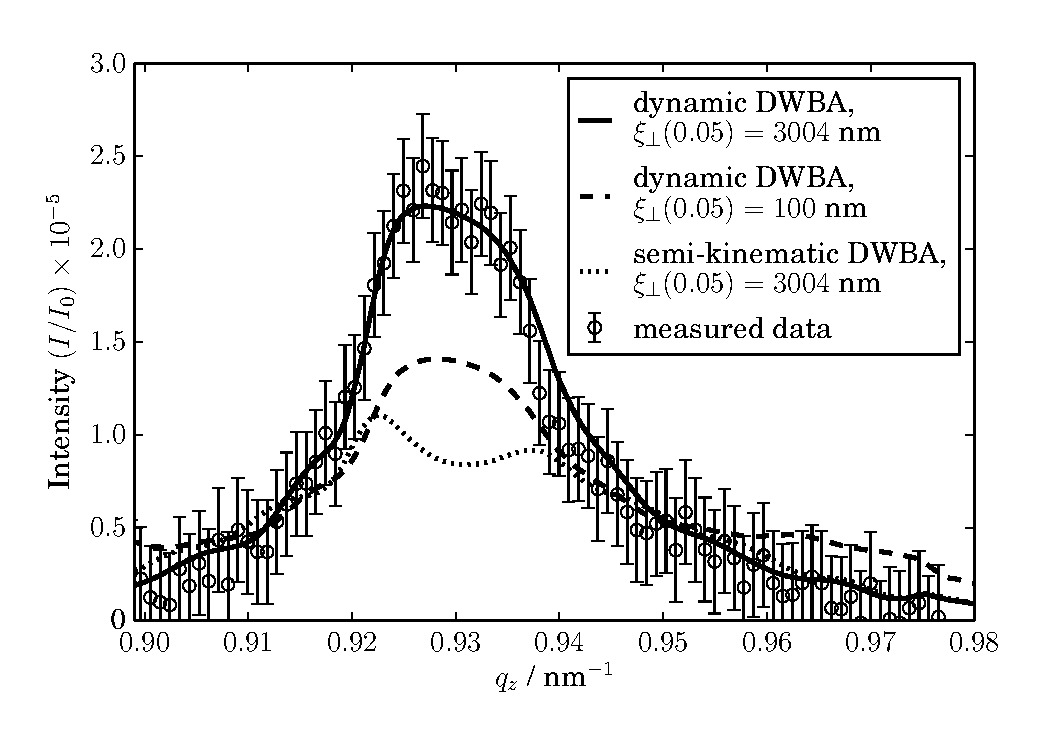
\includegraphics[width=0.5
        \textwidth]{img/im_mo_si/qz_kinematic_vs_dynamic_100nm} \caption{Scattering intensity along $q_z$ for $q_x=0.05$ nm$^{-1}$ for the dynamic and semi-kinematic calculations for a rocking scan at $\Delta\Theta=30^\circ$ in comparison to the measured data.} \label{fig:Comparison_full_semi} 
\end{figure}

To evaluate the contribution of multiple reflections due to the subsidiary maxima, Fig.~\ref{fig:kiessig_like_peak} shows the intensity distribution along $q_x$ at $q_z=0.93$ nm$^{-1}$.  These maxima are caused by interference of the reflections from the top surface of the multilayer stack and the substrate interface (Kiessig fringes) \cite{kiessig1931}.
\begin{figure*}
        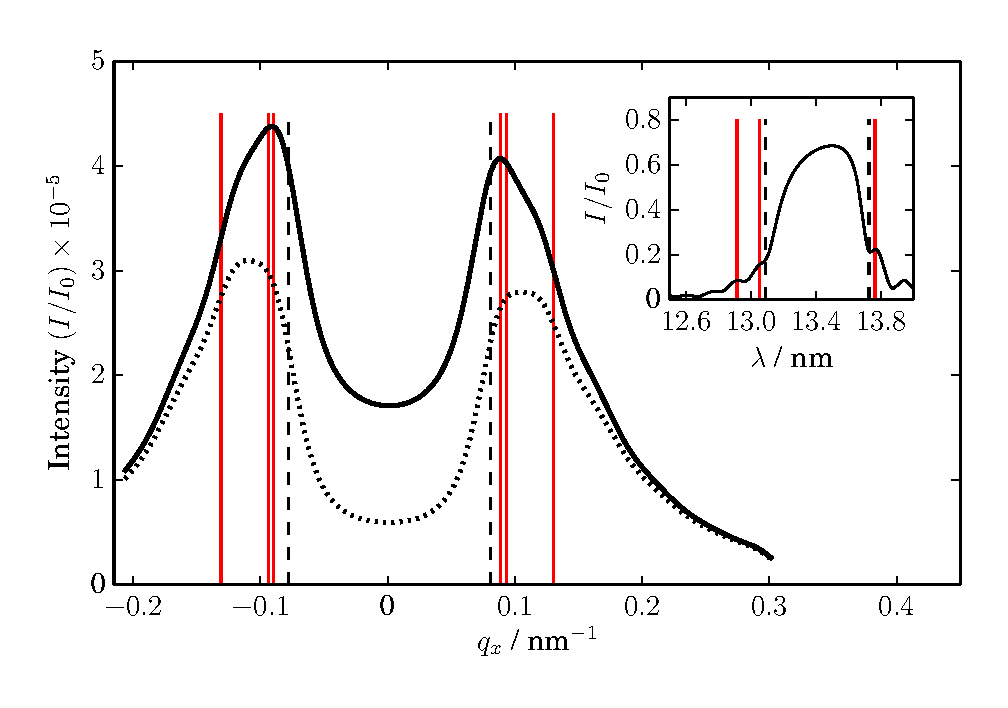
\includegraphics[width=0.5
        \textwidth]{img/im_mo_si/qx_kinematic_vs_dynamic} \caption{Scattering intensity distribution at $q_z=0.93$ nm$^{-1}$. The solid line shows the result of the dynamic calculation for a rocking scan with an opening angle of $\Delta\Theta=30^\circ$. The dashed line represents the calculation applying the semi-kinematic approximation, ignoring any multiple reflections within the multilayer. The dashed vertical lines are the limits of the main Bragg peak, while the red solid vertical lines show the position of dynamic contributions of the Kiessig fringes close to the main maximum. Each Kiessig fringe marked in the inset appears for the corresponding positive and negative $q_x$ value. The strong intensity at $q_x\approx0.1$ nm$^{-1}$ results from the overlap of the dynamic maxima of two different Kiessig fringes (see text).} \label{fig:kiessig_like_peak} 
\end{figure*}
The solid line corresponds to the dynamic theory, while the dotted line is the result of the semi-kinematic calculation. The dashed vertical lines indicate the limits of the main Bragg peak. These positions are defined through the first minimum on each side of the reflectivity peak (cf.~inset in Fig.~\ref{fig:kiessig_like_peak}). The vertical red lines show the position of multiple reflections due to Kiessig fringes close to the main resonance. Again, the corresponding positions in the specular reflectivity measurement are shown in the inset. Each of the marked fringes appears on the negative and positive $q_x$-axis in the main plot. This is caused by the incidence and exit angle, respectively, being at the resonance angle of the various Kiessig maxima in the reflectivity curve. Thus, a strong increase with respect to the semi-kinematic approximation is observed. The position of the dynamic contribution from the first 
Kiessig fringes on either side of the main resonance exhibits a pronounced maximum in the diffuse scattering. These fringes contribute most due to their high overall relative 
intensity compared with the fringes further away from the reflectivity maximum. In addition, the position in reciprocal space coincides with the first two Kiessig fringes marked on either side of the main maximum. This effect of dynamic maxima is similar to the observation of Bragg-like peaks in grazing incidence geometry \cite{PhysRevB.52.16369}, but it is caused by the subsidiary maxima instead. Consequently, we name this enhancement ``Kiessig-like peaks''. The contribution by the main Bragg resonance similar to the observations in Fig.~\ref{fig:Comparison_full_semi} amounts to approximately 100\% at $q_x=0$.

\subsection{Multilayer Enhancement Factor} \label{sec:multilayer_contribution}
The total contribution of the multilayer to the diffuse scattering, independent of lateral interface roughness properties, is described by the sum in the square brackets of Eq.~\eqref{eqn:multilayer_enhancement_factor} as a prefactor to the power spectral density $C(q_x)$. It describes the modulation of the scattering intensity due to the multilayer nature of the scattering structure, independent of the interface roughness. We thus consider it as a ``relative multilayer enhancement factor''. The result of the calculations based on the layer model of our multilayer sample is shown in Fig.~\ref{fig:MultilayerInfluence} for one detector and two rocking scan configurations. The vertical correlation length for this specific multilayer mirror is $\xi_\perp(q_x)=7.5/q_x^2$ nm$^{-1}$ as expected for a high-reflectance mirror, where $\xi_\perp$ 
exceeds the total thickness $D$ of the entire stack for $|q_x| < 0.12$ nm$^{-1}$. The method for the extraction of the vertical correlation length from the measured data is discussed in Sec.~\ref{sec:determination_of_the_psd}. The multilayer enhancement factor was normalized with respect to $q_x=0$, i.e. the calculated diffuse scattering contribution on the specular axis. 
\begin{figure}
        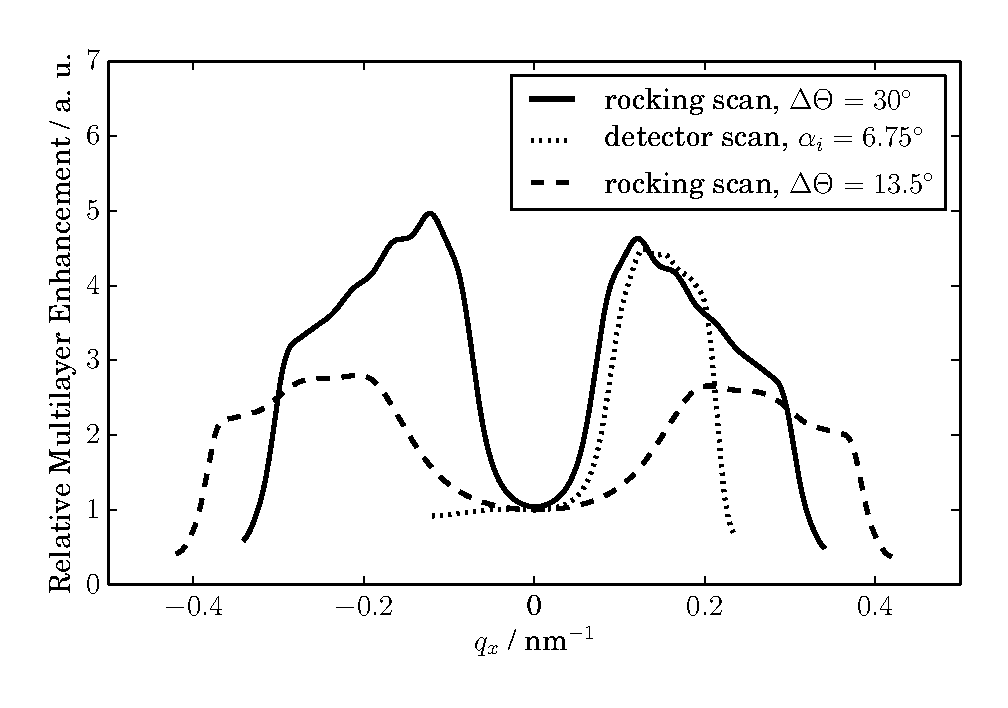
\includegraphics[width=0.5
        \textwidth]{img/im_mo_si/MEF} \caption{Enhancement factor due to the specific properties of multilayer reflectivity for three different measurement geometries. The simulations shown here were normalized with respect to the diffuse contribution to the specular reflectivity at $q_x=0$.} \label{fig:MultilayerInfluence} 
\end{figure}

The results clearly show that diffuse scattering from multilayers at near-normal incidence exhibit strong enhancement due to the intrinsically limited bandpass of reflectivity of multilayers. If both the incidence and exit angle is out of the Bragg resonance, the higher penetration depth of the multilayer causes an increase in the number of interfaces contributing to the diffuse scattering intensity. Thus higher total scattering is observed. The Kiessig fringes cause modulations in the enhancement factor increased by the purely dynamic processes described in Sec.~\ref{sec:dynamic_contributions}.

\begin{figure*}
        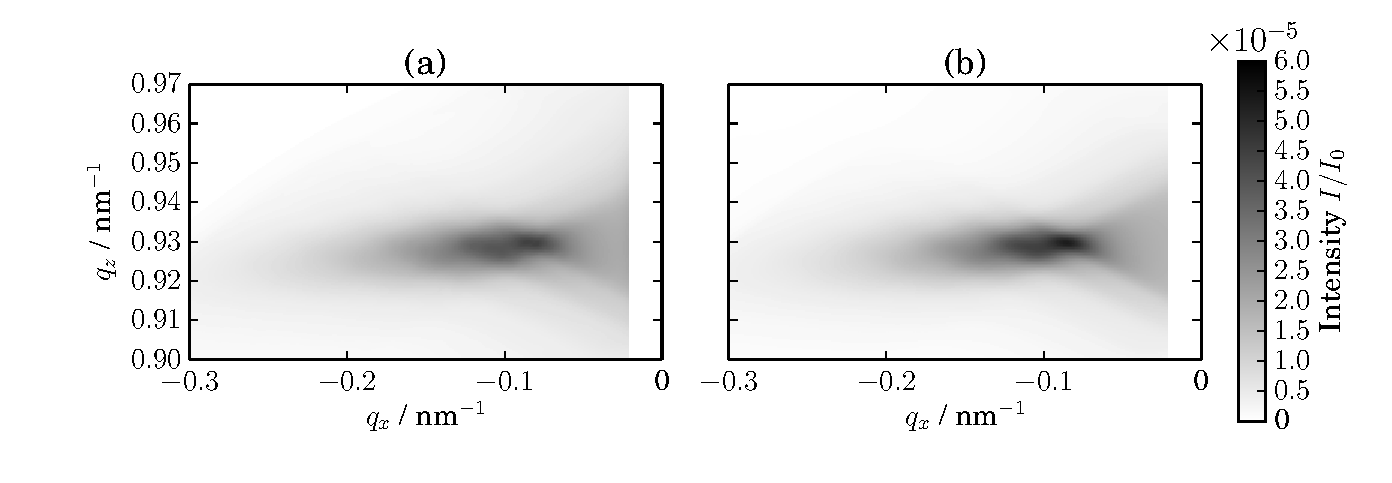
\includegraphics[width=
        \textwidth]{img/im_mo_si/simulation_vs_measurement} \caption{Measured (a) and simulated (b) reciprocal space maps for a rocking scan at an opening angle of $\Delta\Theta=30^\circ$ with the roughness parameters determined in Sec.~\ref{sec:determination_of_the_psd}.} \label{fig:comparisonWithTheory} 
\end{figure*}

\subsection{Reconstruction of the Power Spectral Density} \label{sec:determination_of_the_psd} In order to extract roughness properties from the off-specular measurements shown above, a correction for the influence of the multilayer as discussed in Sec.~\ref{sec:multilayer_contribution} is required. The scattering intensity after division by the multilayer enhancement factor represents the power spectral density of roughness. The measured PSDs are shown in Fig.~\ref{fig:PSDs_linear} for all three experiments. The excellent agreement with each other within the uncertainty margin confirms the validity and necessity of the dynamic theory to model the diffuse scattering from the multilayer. The reconstruction of the parameters of the power spectral density in Eq.~\eqref{eqn:psd} can be done by considering the overall intensity as well as the asymptotic behavior \cite{PhysRevB.54.5860} of the measured data in Fig.~\ref{fig:PSDs_linear}.

The numerical simulations show a strong sensitivity with respect to the mean roughness parameter $\sigma$ through the total portion of diffusely scattered light. As expected for a high-reflectance mirror, we obtained a small roughness value of $\sigma = 0.2$ nm.
\begin{figure}
        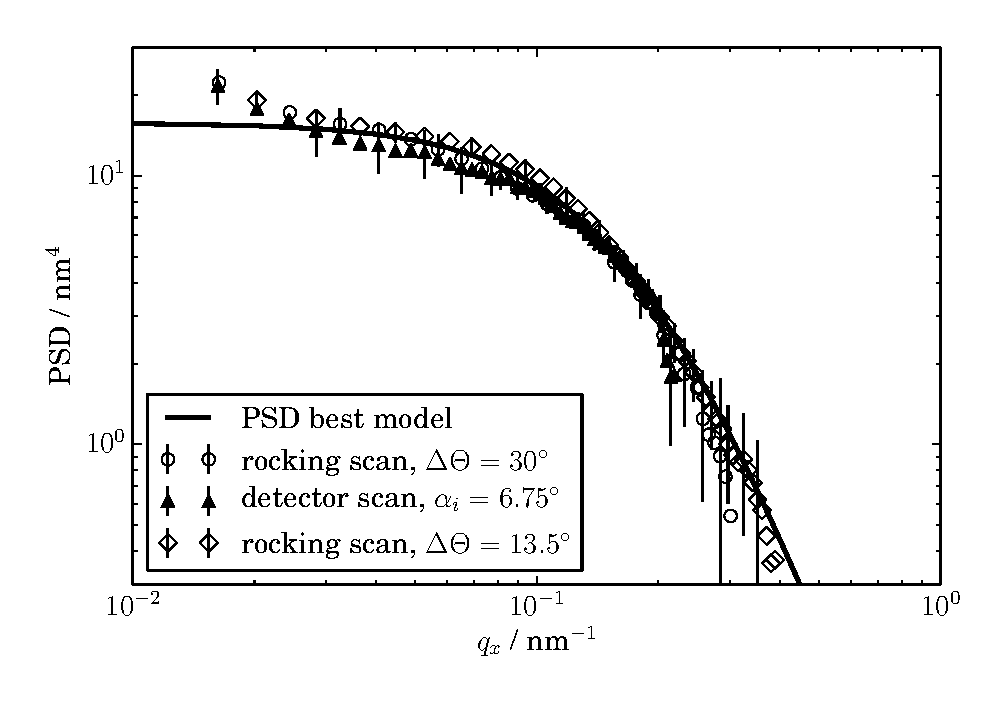
\includegraphics[width=0.5
        \textwidth]{img/im_mo_si/PSD_zoomed} \caption{Diffuse scattering intensity corrected for the multilayer enhancement factor considering a tilt angle of $\beta=-1^{\circ}$ according to Eq.~\eqref{eqn:tilt_correction}. The black solid line corresponds to a power spectral density with $\xi_\parallel=5.6$ nm, $H=1.0$, $\sigma=0.2$ nm and a vertical correlation length of $\xi_\perp(q_x)=7.5/q_x^2$ nm$^{-1}$.} \label{fig:PSDs_linear} 
\end{figure}

It follows from the definition of the PSD in Eq.~\eqref{eqn:psd} that the lateral correlation length $\xi_\parallel$ defines a cut-off for the spatial frequencies contributing to the off-specular scattering. We performed several simulations to compare the simulated intensity profile with the cut-off frequency observed in the measured data. A correlation length of $\xi_\parallel=5.6$ nm was obtained following this method. The fractal nature of the interfaces was analyzed by varying the Hurst parameter $H$. The asymptotic behavior of the power spectral density for $q_x>10^{-1}$~nm$^{-1}$ for the multilayer sample measured yields a Hurst factor of $H=1.0$, which corresponds to a smooth roughness profile \cite{PhysRevB.38.2297}. By following this procedure, measurements of power spectral densities are possible, independent of the measurement geometry.

For a full characterization of the multilayer, the determination of the vertical correlation length remains. This parameter is also accessible through the two-dimensional reciprocal space maps. It has been observed elsewhere that the vertical correlation of the interfacial roughness leads to resonant diffuse scattering (``Bragg sheets'')~\cite{PhysRevB.49.10668}. The width of these sheets with respect to the $q_z$-axis provides a measure for the vertical correlation lengths, e.g.~in GISAXS \cite{Siffalovic200919}. We observe a similar dependence of the scattering intensity close to the Bragg resonance along the vertical axis (cf.~Fig.~\ref{fig:Comparison_full_semi}) with a reduction of the scattering intensity at the resonance for small correlation length but a higher relative scattering intensity far off resonance (cf. $q_z>0.95$ nm$^{-1}$ in Fig.~\ref{fig:Comparison_full_semi}). We varied the vertical correlation length $\xi_\perp(q_x)$ and fitted several vertical cuts of the reciprocal space map 
simultaneously with the PSD determination. The best model for our sample yields a high vertical correlation length of $\xi_\perp(q_x)=7.5/q_x^2$ nm$^{-1}$, as expected for high-reflectance mirrors, at a tilt angle of $\beta=-1^\circ$ of the Bragg plane. 
This correlation length exceeds the total thickness of the multilayer coating up to $|q_x|<0.13$ nm$^{-1}$ and thus indicates (almost) full replication of roughness throughout all interfaces for the specified spacial frequencies.

By combining the findings for the properties of roughness in the power spectral density and the multilayer enhancement factor determined by the layer structure of the multilayer, we are able to fully reconstruct the measured intensity distribution for all geometries. The simulated reciprocal space map for a rocking scan with an opening angle of $\Delta\Theta = 30^\circ$ based on the parameters determined in the previous analysis is shown in Fig.~\ref{fig:comparisonWithTheory}(b). The calculation is in excellent agreement with the measured reciprocal space map in Fig.~\ref{fig:comparisonWithTheory}(a). 


\section{Conclusions} We have applied near-normal incidence diffuse scattering in the EUV spectral range to analyze the interfacial roughness of Mo/Si multilayers. At-wavelength reciprocal space maps in the vicinity of the main Bragg resonance of the multilayer were recorded for the first time via angle and wavelength resolved scatterometry. We observed intensity enhancements in the off-specular scattering. Experiments in different geometries revealed a dependence of the off-specular scattered intensity on the measurement geometry.

Numerical simulations based on the distorted-wave Born approximation (DWBA) have been performed. The comparison of semi-kinematic simulations with dynamic calculations show that dynamic effects, i.e.~multiple reflections at the interfaces, cannot be neglected. The semi-kinematic approach is invalid when either incidence or exit angle fulfill the Bragg condition. In addition, dynamic multiple reflections caused by increased reflectivity due to the Kiessig fringes close to the main Bragg resonance contribute significantly to the off-specular scattering distribution. The simulations show that the limited bandpass reflection property of the multilayer causes the geometry-dependent diffuse scattering in conjunction with the dynamic maxima.

Therefore, in the determination of the interface morphology from co-planar reciprocal space maps a multilayer enhancement factor has to be considered to extract the power spectral density (PSD). We have applied our model to two different measurement geometries with two different angles of incidence for the specular case. Together with the multilayer composition determined from modeled specular reflectivity curves rigorous simulations of the diffuse scattering intensity caused by the multilayer were possible, in excellent agreement with the measured data. The average lateral power spectral density could then be extracted with regard to the multilayer enhancement factor equivalently for any measurement geometry. In addition, measurements along the $q_z$ direction provide information on the vertical correlation of interfaces, i.e.~the determination of the vertical correlation length. 

In conclusion, the consideration of the dynamic effects in the DWBA allows the characterization of the multilayer with respect to its roughness properties. The diffuse scattering measurements corrected for the multilayer enhancement factor provide a measure of the power spectral density. Thus, this method is not restricted to the specific representation of the power spectral density used in our model. Alternative power spectral density models have been discussed in the literature \cite{PhysRevB.38.2297, PhysRevB.48.2873} and are equivalently applicable in the numerical simulations.

    \chapter{Characterization of sub-nanometer Cr/Sc Multilayer Systems}

\section{Introduction}

The wavelength range of the so called ``water window'' between $2.2$ nm and $4.4$ nm wavelength is of special interest for many scientific applications. Radiation in this spectral range shows low absorption in water, while it is absorbed by many elements naturally occurring in organic molecules such as proteins \cite{WaterWindowBioRelevance}. This allows to study those biological systems in water, where many proteins are biologically active. High-reflective optics are required to take advantage of the high resolution possible due to the short wavelength in direct imaging of these samples \cite{waterwindow_mirrors_1,Legall:12}.

The strong absorption of soft X-ray radiation in most materials poses a challenge in the fabrication of such optics. Refractive optics are almost impossible due to the high absorption in solids. The same holds for reflective optics close to normal incidence, where reflectivities of well below $10^{-4}$ can be expected from a single surface of all materials \cite{henke}. A candidate system for building high-reflective mirrors for short wavelength is a layered structure with alternating materials of significantly different refractive index \cite{SpillerMultilayer}. Those multiple repeated bilayer systems constitute an artificial one-dimensional Bragg crystal. Their layer layout, more specifically the total layer thickness $D$ of a single layer period, is intrinsically related to the desired peak reflectivity wavelength and incidence angle. Those systems are well established as mirrors for EUV wavelength of $13.5$ nm, where they reflect more than $70\%$ of the radiation at angles of incidence of $6^\circ$ from 
the surface normal with a choice of Mo and Si as layer materials. Theoretical calculations show that constructing multilayer mirrors in the water window spectral range for angles of incidence of $1.5^\circ$ allows peak reflectivities above $50\%$ \cite{Schafers:98}. A typical choice of materials for these bilayer systems are Cr and Sc for wavelength above $3.1$ nm \cite{Salashchenko19977, Schafers:98}. The proximity to the Sc L-edge causes the required significant difference in the refractive index due to anomalous dispersion while maintaining relatively low absorption. In order to function as a one-dimensional Bragg crystal those layer systems demand a high quality of the layer interfaces. Chemically abrupt and smooth interfaces are required to reach high reflectivities and to minimize loss processes such as diffuse scattering or contrast decrease due to interdiffusion. This requirement becomes even more stringent when moving towards shorter wavelength due to the necessary reduction in layer thickness for 
fulfilling the Bragg condition.
The relative influence of interface morphology and interdiffusion as loss mechanisms for peak reflectivity rise in importance compared to established Mo/Si multilayer systems with significantly larger layer thicknesses. The measured peak reflectivity of state-of-the-art Cr/Sc multilayer systems designed for the above specifications score at reflectivities below $20\%$, less than half of the theoretically possible value (cf.~inset~Fig.~\ref{fig:EUV_XRR_reflectivity}) \cite{Eriksson:03, doi:10.1117/12.505688}.

Roughness causes diffuse scattering out of the specular beam direction \cite{sinha_scattering_natural_tool}. Interdiffusion on the other hand reduces the optical contrast, i.e.~the local difference in the refractive index thereby reducing the reflectivity at each interface \cite{nakajima_interdiffusion}. In order to gain a deeper understanding of the interface morphology a characterization of these samples is required. The inspection of diffusely scattered light is a natural tool for the investigation of the roughness at the interfaces. An at-wavelength measurement of in-plane diffuse scattering contributions contains information on the interface morphology. An important advantage of this analysis as compared to established methods for interface characterization of thin films such as GISAXS \cite{Levine:pn0068} is that the angle of incidence is close to the surface normal. This enables the possibility to locally investigate the multilayer stack even for strongly curved surfaces, e.g.~in case of focusing 
optics.


Standard characterization methods such as EUV reflectivity and X-ray reflectivity with simple binary layer models have proven useful for the characterization of similar multilayer systems, e.g.~Mo/Si mirrors designed for $13.5$ nm wavelength \cite{Lim2001, bajt_mosi_crstallization, braun_mosi_different_barrier_layers}. However, these systems typically have thicknesses of $3$ -- $4$ nm within a single period for the Mo and Si layers. With the efforts of reducing the desired peak reflectivity wavelength, those methods fail in yielding information to build simple models that describe measured reflectivities \cite{Yakunin:14}. The results of the analysis based on the standard binary model of a Cr/Sc multilayer with a Sc to Cr ratio of $\Gamma_\text{Sc}=0.48$ are shown in Fig.~\ref{fig:EUV_XRR_reflectivity}. The individual layer thicknesses for this sample were fitted to be $d_\text{Cr} = 0.81$ nm and $d_\text{Sc}= 0.75$ nm. While the EUV reflectivity curve (cf.~inset in Fig.~\ref{fig:EUV_XRR_reflectivity}) shows 
a good agreement with the measured data, there is a significant offset in case of the XRR measurement with the (binary) model derived from the EUV reflectivity experiment. Even a simultaneous analysis could not yield a consistent result. In a strictly binary model with a layer thickness ratio of $\Gamma_\text{Sc}\approx 0.5$, the second Bragg peak is suppressed due to symmetry reasons. This, however, is a clear mismatch with the experimental observation as seen in the comparison of the fitted and measured XRR curves in Fig.~\ref{fig:EUV_XRR_reflectivity}.
\begin{figure}
  \centering
  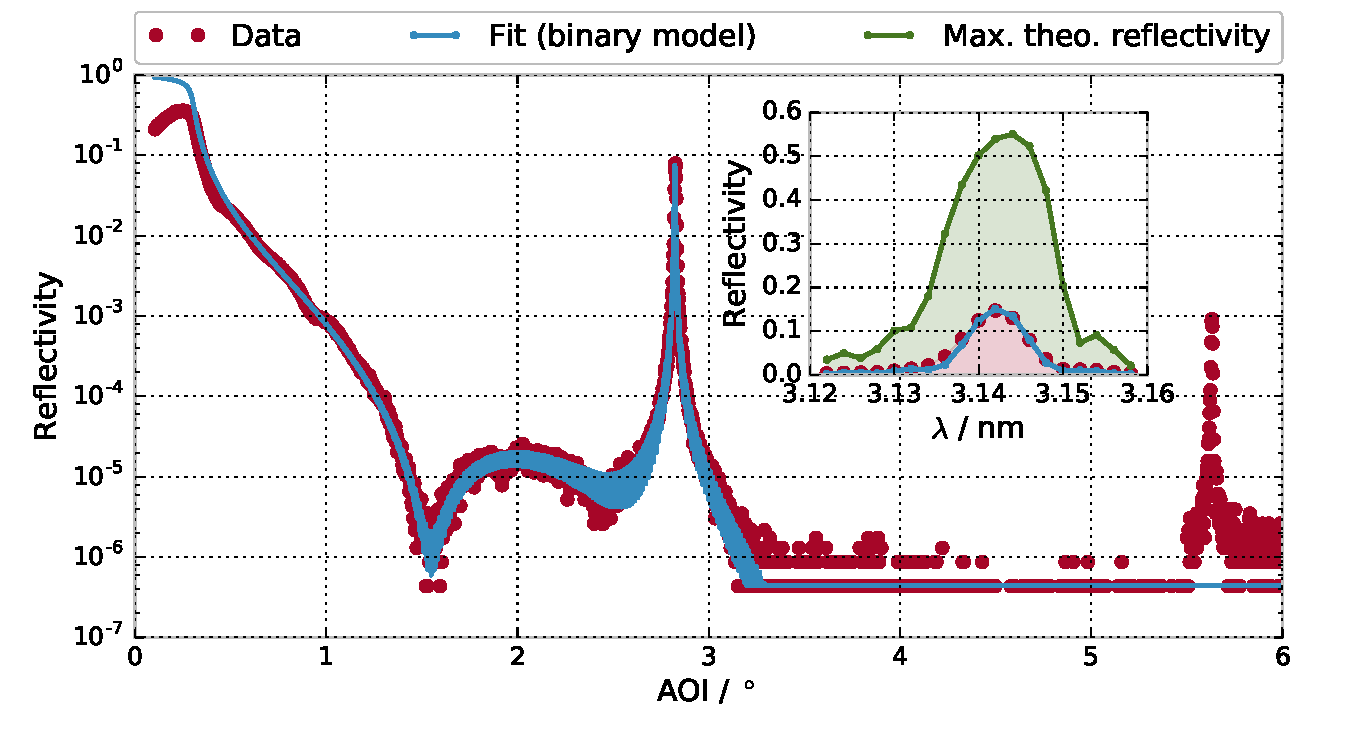
\includegraphics[width=\textwidth]{img/im_cr_sc_multilayer/binary_model_and_theo_refl}
  \caption{Theoretical and experimental X-ray reflectivity curves based on the simple binary model. The optimal model based on the analysis of the EUV reflectivity (cf.~inset) shows a clear mismatch with the measured XRR curve in the second Bragg peak. Inset: Fitted experimental EUV reflectivity curves across the wavelength of the radiation impinging at $1.5^\circ$ from normal based on a simple binary model. The green curve shows the maximum possible reflectivity assuming a perfect layer system.
}
  \label{fig:EUV_XRR_reflectivity}
\end{figure}

The reason for this mismatch is the growing relative influence of disturbances at the interfaces potential breaking the symmetry condition. This needs to be taken into account explicitly in the model and leaves the simple binary approach as an insufficient description of the physical situation. The increase of parameters required to describe a more realistic model also pose a requirement on information gained through analytic experiments. We thus apply a set of different experimental methods to obtain a consistent reconstruction of the multilayer structure with a non-destructive approach. We demonstrate that in case of layer systems in the sub-nanometer regime, a combined analysis of this experiments is required. For this, we derive a sophisticated model considering graded interface profiles and intermixing of the two materials. The validation of the derived model is conducted by applying a Markov-chain Monte Carlo sampler.



\section{Experimental details} \label{sec:experimental}

The multilayer samples were prepared at the DESY X-ray multilayer laboratory by DC magnetron sputtering \cite{crsc_thermal_bajt} \todo{more info}. They are composed out of alternating layers of Cr and Sc with periodic replication of the bilayer stack by $N=400$ times. The substrates are superpolished Si wafer pieces. The sample dimensions measure approximately $(20 \times 20)$ mm$^2$. The multilayer mirrors were designed to reflect radiation in the water window energetically below the Sc L-edge close to $3.1$ nm wavelength at an angle of incidence of $1.5^\circ$ from the surface normal.

The characterization via XRR was conducted in the DESY laboratory using a high-resolution X-ray diffractometer. It is equipped with a high-resolution goniometer and uses the Cu-K$_\alpha$ wavelength. The reflectivity experiments were recorded using a counting detector in grazing incidence geometry measured at angles of incidence from $\alpha_i=0^\circ$ to $\alpha_i=3^\circ$. The dynamic range achieved in the measurement ranged down to a reflectivity of $10^{-6}$. Due to the low layer thickness in each period of the multilayer sample, only two Bragg peaks at most could be measured with this technique. All higher order peaks were below the detection threshold of $10^{-6}$ in reflected intensity.

All other experiments were conducted in the laboratory of the Physikalisch-Technische Bundesanstalt (PTB) at the electron storage ring BESSY II in Berlin-Adlershof. The EUV reflectivity (cf.~inset Fig.~\ref{fig:EUV_XRR_reflectivity}) and resonant EUV reflectivity measurements (REUV, cf.~Fig.~\ref{fig:REUV_XRF_data}(a)) were done in the new ellipso-scatterometer at the soft X-ray beamline \cite{Beckhoff2009} under ultra high vacuum (UHV) conditions. The accessible spectral range at the SX700 plane grating monochromator ranges from $0.8$ nm to $25$ nm. The samples were mounted on a 6-axis goniometer sample holder. The movable detector arm in combination with the goniometer allows measurements in in-plane and out-of-plane geometry. For the resonant EUV (REUV) reflectivity measurements across the Sc L-edge the wavelength was kept fixed while performing a specular angular reflectivity scan ($\Theta$/$2\Theta$-scan). The X-ray standing wave experiments or X-ray flourescence experiments (XSW/XRF), respectively, 
were done at the four-crystal monochromator beamline (FCM), where energies up to $10$ keV well above the K-absorption edges of Sc and Cr are accessible. The end station is a dedicated X-ray flourescence measurement chamber also under UHV. The fluorescence data was taken at a selected photon energy of $E=6.25$ keV, above the Cr edge. The relative fluorescence yield from the Sc and Cr K-edges, respectively, is shown in Fig.~\ref{fig:REUV_XRF_data}(b) and~\ref{fig:REUV_XRF_data}(c). The grazing angle of incidence was varied across the resonance condition for the first Bragg peak to excite the standing wave field inside the multilayer.
\onecolumn
\begin{figure}
  \centering
  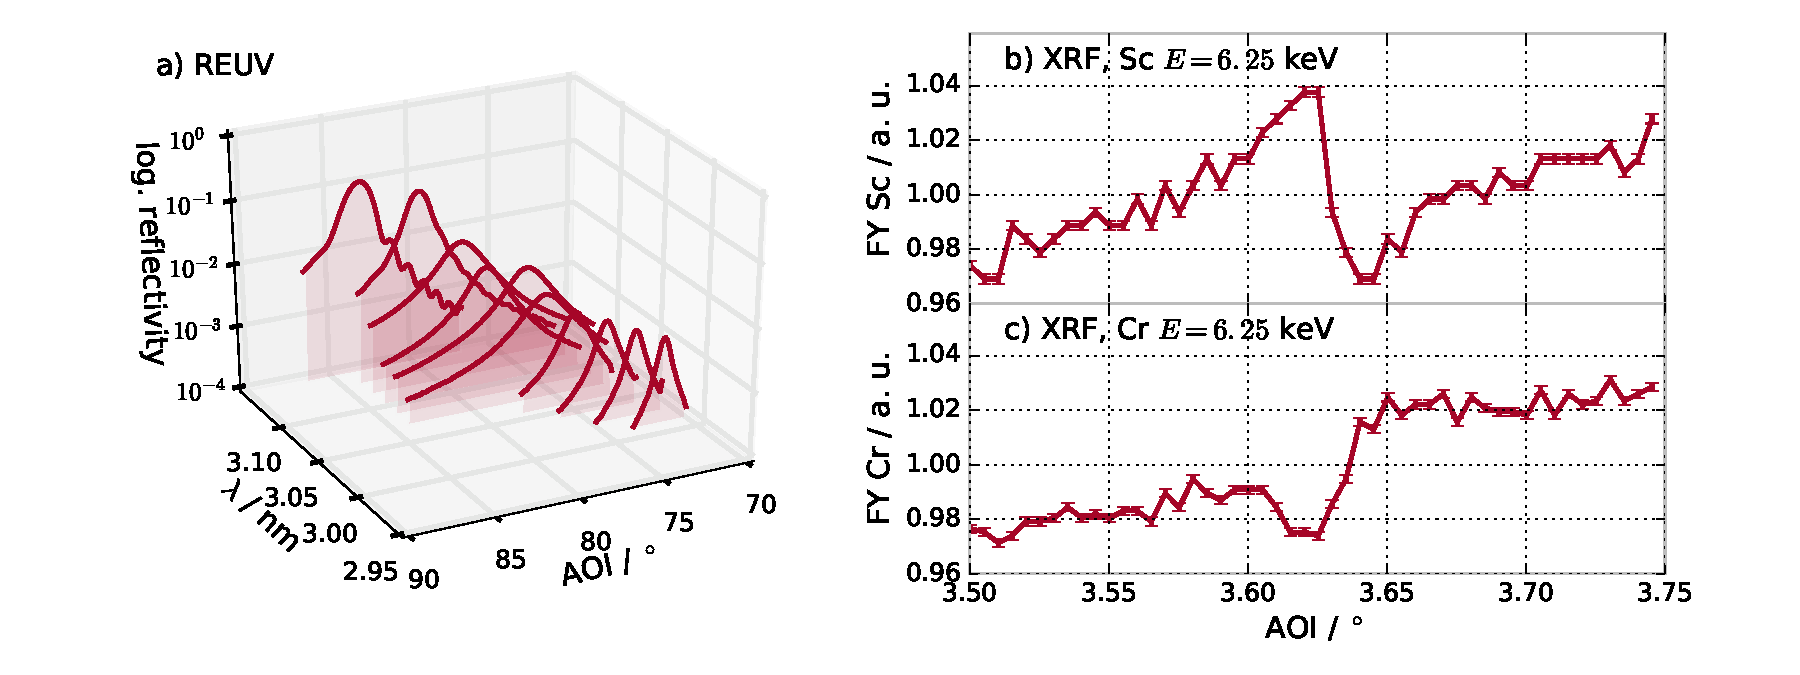
\includegraphics[width=\textwidth]{img/im_cr_sc_multilayer/reuv_xrf_data}
  \caption{a) Resonant EUV reflectivity across the Sc L-edge. Several angular reflectivity scans have been performed at selected wavelength across the Sc L-edge. b) and c) X-ray standing wave fluorescence recorded across the first Bragg peak by varying the angle of incidence for the Sc signal (b) and the Cr signal (c). Both curves were recorded simultaneously at an excitation energy of $E=6.25$ keV. The data is shown in relative (arbitrary) units of intensity.}
  \label{fig:REUV_XRF_data}
\end{figure}


The diffuse scattering measurements were performed with a detector angle of $2\Theta = 3^\circ$ with respect to the incoming beam, while rocking the sample from $\Theta = 1.5^\circ - 7.0^\circ$ and tuning the wavelength from $\lambda = 3.0 - 3.4$ nm at each angular position. Diffuse scattering measurements close to near-normal incidence allow for local measurements due to the small beam spotsize on the sample. This measurement technique allows to obtain a reciprocal space map of the diffuse scattering distribution as shown in Fig.~\ref{fig:diffuse_meas} below.


\section{Theoretical background} \label{sec:matrix_formalism}

\subsection{Matrix formalism: EUV, REUV, XRR} \label{subsec:matrix_formalism}

The EUV and X-ray reflectivity is calculated based on the well established matrix formalism \cite{PrinciplesOfOptics}. The reflection $r_{id}^{(j)}$  and transmission $t_{id}^{(j)}$ at each interface $j$ is given by the Fresnel coefficients
\begin{align}
        r_{id}^{(j)} &= \frac{k_z^{(j)} - k_z^{(j+1)}}{k_z^{(j)} + k_z^{(j+1)}}\text{,} \\
        t_{id}^{(j)} &= \frac{2 k_z^{(j)}}{k_z^{(j)} + k_z^{(j+1)}}\text{,} 
\end{align}
where $k_z^{(j)}$ is the complex $z$-component of the incident wave vector $\vec{k}$ at the $j$th interface. Its value is calculated according to Snell's law at each interface taking into account the complex indices of refraction $n^{(j)}$.
In order to account for roughness induced loss of specular reflectivity, modified Fresnel coefficients based on a Nevot-Croce factor $\sigma_r$ are considered at each interface \cite{nevot_croece}. We approximate the interface mean square roughness to be identical at each interface, i.e.~$\sigma_j \equiv \sigma_r\text{,} \, \forall j$. Considering different roughness at each interface would increase the number of variable parameters in the model by the amount of interfaces and thus lead to overdetermination. The analysis of the diffuse scattering from Mo/Si multilayer systems has shown a high correlation of the interface roughness throughout the stack \cite{Haase:14}, which supports the approximation of identical roughness made here. With this approximation the modified Fresnel coefficients assuming a error function type interface profile are given by
\begin{align}
        r^{(j)} &= r_{id}^{(j)} \exp(-2 k_z^{(j)} k_z^{(j+1)} \sigma_r^2)\text{,} \nonumber \\
        t^{(j)} &= t_{id}^{(j)} \exp((k_z^{(j)} - k_z^{(j+1)})^2 \sigma_r^2/2) \text{.} \label{eqn:modified_fresnel}
\end{align}

The electric fields at each interface are then related with the fields at the next interface through the field propagation matrix $M_j$ \cite{mikulik1997x}
\begin{align}
M_j = \frac{1}{t^{(j)}}
\begin{pmatrix}
1 & r^{(j)} \\
r^{(j)} & 1
\end{pmatrix}
\begin{pmatrix}
e^{-i k_z^{(j+1)} d_j} & 1 \\
1 & e^{i k_z^{(j+1)} d_j}
\end{pmatrix}
\text{,} \label{eqn:field_propagation_matrix}
\end{align}
The fields inside the multilayer stack, as well as inside the substrate and the vacuum are given by Eq.~\eqref{eqn:field_propagation_equation}.
\begin{align}
\begin{pmatrix}
E_0 \\
E_R
\end{pmatrix} &=
\prod\limits_{j} M_j
\begin{pmatrix}
E_T \\
0
\end{pmatrix} \text{.} \label{eqn:field_propagation_equation}
\end{align} 
The total wave field is represented by a two dimensional vector. The upper component describes the amplitude of the wave propagating towards the substrate and the lower component describes the reflected wave amplitude propagating towards the vacuum. Iterative application of the field propagation matrix yields the electric field amplitudes $E$ at each interface for both propagation directions. The solution is obtained by starting from the condition of a known incoming wave amplitude $E_0$ and the lack of a reflected wave amplitude inside the substrate.

The components $E_T$ and $E_R$ describe the transmitted and reflected field amplitudes inside the vacuum and the substrate, respectively.
Normalized reflectivity $R$ and transmitivity $T$ values for the EUV, REUV and XRR measurements are obtained from the field calculation by dividing the calculated values with the initial field amplitude $E_0$
\begin{align}
R &= |E_R/E_0|^2\text{,} \nonumber\\
T &= |E_T/E_0|^2 \text{.} \label{eqn:refl_trans}
\end{align}

\subsection{X-ray standing wave fluorescence analysis} \label{subsec:xrf_formalism}

The calculation of the relative fluorescence signal XRF for either element in the multilayer stack is done by discrete numerical integration of the product of the total electric field intensities $I \propto |E(z)|^2 = | E_r(z) + E_t(z)|^2$ with the relative density profile of the elements $\rho(z) = \rho_\text{Sc}(z)$ or $\rho(z) = \rho_\text{Cr}(z)$, respectively, along the surface normal of the sample, i.e.~
\begin{align}
 I_\text{XRF}\propto \int\limits_0^{D_\text{total}} |E(z)|^2 \rho(z) \,\text{d}z \text{,}
\end{align}
where the total thickness $D_\text{total}$ of the multilayer stack is given by $D_\text{total} = N D+D_\text{cap}$ with $N$ being the number of multilayer periods, $D$ the thickness of a single period and $D_\text{cap}$ the total tickness of all capping layers and $z$ is the coordinate along the surface normal with respect to the substrate surface. The total electric field $E(z)$ is evaluated at discrete points $z_j$ inside the multilayer including the interfaces according to Eq.~\eqref{eqn:field_propagation_equation}, while the distance between two sample points is significantly less than the thickness of a single layer to approximate the continous wave intensity dependence along $z$.
\subsection{Distorted-wave Born approximation} \label{subsec:dwba_formalism}

The theoretical analysis of the diffuse EUV scattering data obtained has been done based on the distorted-wave Born approximation (DWBA) \cite{PhysRevB.49.10668,PhysRevB.47.15896}. Here, the interface roughness is considered to be a small distortion on the solution of the perfect multilayer system. We apply that to diffuse scattering measurements near-normal incidence, where dynamic effects become important and need to be considered in order to obtain the power spectral density (PSD) of the interface morphology. Our approach is described in detail in \cite{haase_role_2014}. Following from Eq.~\eqref{eqn:field_propagation_equation} and Eq.~\eqref{eqn:refl_trans} The explicit transmitted and reflected fields at the interfaces are given by
\begin{align}
        E_t^{(j)}(z) &= T_{j} e^{i k_z^{(j)} z} \text{,} \\
        E_r^{(j)}(z) &= R_{j} e^{-i k_z^{(j)} z} \text{,}
\end{align}
where $T_{j}$ and $R_{j}$ are the transmitted and reflected field amplitudes at each interface, respectively. The fields are calculated based on the matrix formalism described above using the undisturbed system, i.e.~the ideal Fresnel coefficients instead of the modified coefficients already including a correction for roughness. The solution serves as the undisturbed wave field entering the DWBA calculation. The diffuse scattering intensity is then given by
\onecolumn
    \begin{align}
        \Big(\frac{d \sigma}{d \Omega}\Big) = &\Bigg[\frac{A \pi^2}{\lambda^4}\sum \limits_{j=1}^{N}\sum \limits_{i=1}^{N} (n_j^2 - n_{j+1}^2)^* (n_i^2 - n_{i+1}^2)\Big( (T^{(1)}_j + R^{(1)}_j)^* (T^{(2)}_j + R^{(2)}_j)^* \nonumber \\ &\qquad\times(T^{(1)}_i + R^{(1)}_i) (T^{(2)}_i + R^{(2)}_i) \Big) \exp\Big(-i q_x \tan \beta (z_i-z_j)\Big) c^\perp_{i j}\Bigg]\,\, C(q_x) \text{,} \label{eqn:dwba}
    \end{align}

taking into account all first-order dynamic effects. Here, $n_j$ represents the complex refractive index inside each layer, $A$ respresents the illuminated area, $\lambda$ respresents the wavelength of the impinging radiation, $\beta$ indicates the angle at which correlated roughness replicates from interface to interface throughout the stack and $z_i$ the position of the interface, both with respect to the surface normal. The leading term of Eq.~\eqref{eqn:dwba} contained within rectangular brackets can be considered as a multilayer enhancement factor separating the contributions of the multilayer nature and the vertical correlations of the sample from the roughness at the interfaces isolated in the PSD $C(q_x)$. The scattering distribution is calculated in reciprocal space coordinates or the wave vector transfer $q$ given by
\begin{align}
        q_x &= \frac{2 \pi}{\lambda} \big(\sin(\alpha_f) - \sin(\alpha_i)\big) \text{,}\\
        q_z &= \frac{2\pi}{\lambda} \big(\cos(\alpha_f) + \cos(\alpha_i)\big) \text{,} 
\end{align}
where $\alpha_i$ is the angle of incidence from normal and $\alpha_f$ is the scattering angle.
The roughness properties of the interfaces is contained in the replication factor $c_{ij}^\perp$ \cite{spiller1993multilayer} and the effective one-dimensional power spectral density $C(q_x)$. There exist several PSD models in literature, e.g.~by Sinha et al.~\cite{PhysRevB.38.2297}, for single rough interfaces or surfaces, respectively. Due to the low thickness of the individual layers we make the approximation of identical statistical properties of each interface with respect to the roughness, i.e.~we assume identical PSDs. We follow the definition of de Boehr et al.~\cite{deBoerLateralCorrelation,PhysRevB.51.5297} which yields a closed analytic form of the PSD for a fractal roughness model
\begin{align}
    C(q_x) = \frac{4 \pi H \sigma_r^2 \xi_\parallel^2}{(1+|q_x|^2\xi_\parallel^2)^{1+H}} \text{,} \label{eqn:psd} 
\end{align}
where $\sigma_r$ is the root mean square roughness, $H$ is the Hurst factor describing the jaggedness of the interface and $\xi_\parallel$ is the in-plane correlation length. The replication factor $c_{ij}^\perp$ is given by
\begin{align}
c_{ij}^\perp(q_x) =  \exp\Bigg(-\sum \limits_{n = \text{min}(i,j)}^{\text{max}(i,j)-1}d_n/\xi_\perp(q_x) \Bigg)\text{,}
\end{align}
where $d_n$ is the thickness of the $n$th layer and $\xi_\perp(q_x) = \xi_\perp/q_x^2$ is a spacial frequency dependent vertical correlation length at which the replication factor has decreased to $1/e$.


\section{Improved model for robust reconstruction} \label{sec:model}

Instead of the simple binary layer model a gradual interface model is introduced to better reflect the realistic electron density profile due to interdiffusion and roughness. A corresponding profile is shown in Fig.~\ref{fig:CrScModel} for illustration in comparison to the binary model.
\begin{figure*}
  \import{svg/CrSc_model.pdf_tex}
  \caption{a) Binary Cr/Sc multilayer model with total period thickness $D$ and the individual layer thicknesses $d_\text{Sc}$ and $d_\text{Cr}$. b) Gradual interface model with explicit gradual interfaces following a sinusoidal profile. The ideal interface profile is approximated through discrete sublayers as indicated in red forming the actual gradual interface profile entering the electric field calculations. The thickness of the interdiffusion zones can differ for the top and bottom interface in each period. Their total thicknesses is given by $s_\text{Sc}$ and $s_\text{Cr}$. Due to intermixing across multiple periods a reduction of the index of refraction for each material towards the average of both materials is possible. The effective index of refraction for both materials is thus given by $\tilde{n}_\text{Sc}$ and $\tilde{n}_\text{Cr}$, respectively.}
  \label{fig:CrScModel}
\end{figure*}
The calculation of the electromagnetic fields is then conducted based on this model with the matrix formalism introduced in the preceding section. The interface region with sinusoidal profiles is sampled with a fixed number of equally spaced points in $z$-direction effectively creating a region of thin sublayers with gradually changing index of refraction. The parameters of our multilayer model are listed in Table~\ref{tbl:parametrization},
\begin{table}
\centering
\caption{Multilayer parametrization and parameter limits}
\label{tbl:parametrization}
\begin{tabular}{@{}llll@{}}
\toprule
Parameter & Definition & Lower bound & Upper bound\\ \midrule
$D$ / nm & $= d_\text{Sc} + d_\text{Cr}$ & 1.5&1.6 \\ 
$\Gamma_{Sc}$ & $= d_\text{Sc} / D$&0.0 &1.0 \\ 
$\sigma_d$ / nm&$=s_\text{Sc} + s_\text{Cr}$&0.0 & 1.6\protect\footnotemark\\ 
$\Gamma_\sigma$ &$= s_\text{Sc} / \big(s_\text{Sc} + s_\text{Cr}\big)$& 0.0& 1.0\\ 
$\eta$ &layer intermixing& 0.0& 1.0\\ 
$\sigma_r$ / nm & r.m.s.~roughness& 0.0& 0.5\\ 
$\rho_{Sc}$ &Sc density w.r.t.~bulk density & 0.5& 1.0\\ 
$\rho_{Cr}$ &Cr density w.r.t.~bulk density& 0.5& 1.0\\ 
 \bottomrule
\end{tabular}
\end{table}
\footnotetext{The maximum value of the interdiffusion layer thickness is limited due to the thicknesses of the individual layers $d_\text{Sc}$ and $d_\text{Cr}$ through the relation $\sigma_d \leq D$}
%\begin{align}
%       \text{Multilayer parametrization}
%    \begin{cases}
%       D &= d_\text{Sc} + d_\text{Cr}\\
%        \Gamma_\text{Sc}  &= d_\text{Sc} / D\\
%        \sigma_\text{diff} &=\sigma_\text{Sc} + \sigma_\text{Cr}\\
%        \Gamma_\sigma &= \sigma_\text{Sc} / \big(\sigma_\text{Sc} + \sigma_\text{Cr}\big) \\
%        \eta &\text{layer intermixing} \\
%        \sigma_\text{rough} \\
%        \rho_\text{Sc}\\
%        \rho_\text{Cr}
%    \end{cases} \text{,} \label{eqn:parametrization}
%\end{align}
where $D$ is the full period thickness, $d_\text{Sc}$ and $d_\text{Cr}$ are the nominal layer thicknesses of the Cr and Sc layers as indicated in Fig.~\ref{fig:CrScModel} and $\rho_\text{Sc}$ and $\rho_\text{Cr}$ their respective densities. The parameters $s_\text{Sc}$ and $s_\text{Cr}$ describe the full width of the interdiffusion layers as shown in Fig.~\ref{fig:CrScModel}. To take into account intermixing extending across the full period, we introduced an intermixing parameter $\eta$. The effective indexes of refraction of the individual Cr and Sc layers are then given through
\begin{align}
\tilde{n}_\text{Sc} &=(\eta/2) n_\text{Sc} + (1-\eta/2) n_\text{Cr} \text{,} \nonumber\\
\tilde{n}_\text{Cr} &=(1-\eta/2) n_\text{Sc} + (\eta/2) n_\text{Cr} \text{,} \label{eqn:effective_n} \\
&\text{for} \quad \eta \in [0,1] \text{,}\nonumber
\end{align}
where $n_\text{Cr}$ and $n_\text{Sc}$ are the tabulated values \cite{henke} with densities $\rho_\text{Cr}$ and $\rho_\text{Sc}$. The loss of specular reflectivity due to roughness induced scattering is considered through the Nevot-Croce factor $\sigma_\text{r}$ identical at each interface for the reasons described in above section. To improve the optimization procedure and to reduce correlations between individual parameters, we have selected some effective parameters as defined in Table~\ref{tbl:parametrization}. The parameter $\Gamma_\text{Sc}$ indicates the portion of the Sc layer thickness with respect to the full period thickness $D$, $\Gamma_\sigma$ describes the asymmetry of the extend of the sinusoidal profiles at the Cr/Sc and Sc/Cr interfaces and is limited to the interval $\Gamma_\sigma \in [0,1]$. In addition we restrict the sum of both interface profile extents to the total layer thickness, i.e.~$\sigma_\text{Sc} + \sigma_\text{Cr} \leq D$. This is without loss of generality due to the 
intermixing parameter, which allows for a reduction of the index of refraction w.r.t.~the bulk Sc and Cr layers. This describes a situation, where only interface layers exist due to strong intermixing.

%Each of the interface regions was sampled with 15 points, effectively leading to 15 additional sublayers. Increasing the number of sublayers has led to no improvement of the accuracy of the electric field calculations. In case of the X-ray fluorescence calculations, all layers are sampled in this way.


\section{Combination of EUV, REUV, XRR and XRF}

The reconstruction of the multilayer structure has been conducted with a series of experiments. The minimization functional of the combined analysis $\chi^2$ of the optimization problem is defined as the sum of the least-square functionals for each experiment,
\begin{align}
\chi^2_\text{tot} = \chi^2_\text{EUV} +\chi^2_\text{XRR} +\chi^2_\text{REUV} + \chi^2_\text{XRF}\text{,} \label{eqn:total_chi_2}
\end{align}
where each of the functionals is defined as
\begin{align}
\chi^2 = \frac{1}{m - p} \bigg[\sum\limits_{m} \frac{(I_\text{model} - I_\text{meas})^2}{\tilde{\sigma}^2} \bigg] \text{.}
\end{align}
With $m$ being the number of measurement points in each experiment and $p$ the number of parameters for the model. Statistical and systematic uncertainties for each data point are included in $\tilde{\sigma}$. The definition of Eq.~\eqref{eqn:total_chi_2} ensures that all experiments are weighted equally considering their respective uncertainties.

The minimization is performed with a particle-swarm optimizer (PSO) \cite{Kennedy2010}. In case of an optimization problem with many local minima, this provides an advantage with respect to gradient methods, where the fit result is dependent on the choice of starting values. Similar approaches employing genetic algorithms for solving the inverse problem of scatterometry can be found in literature \cite{del2000modeling}. In case of the model parametrization given in Sec.~\ref{sec:model}, the choice of the parameter intervals is defined either by physical plausability or the fact that the parameter is intrinsically defined in a certain interval as for the intermixing $\eta$, for example. The intervals used in our analysis are listed in Table \ref{tbl:parametrization}.
% \begin{table}
% \centering
% \caption{Intervals of the parameters entering the PSO procedure}
% \label{tbl:intervals}
% \begin{tabular}{@{}lll@{}}
% \toprule
% Parameter & Lower bound & Upper bound\\ \midrule
% $D$ / nm & 1.5&1.6 \\ 
% $\Gamma_{Sc}$ &0.0 &1.0 \\ 
% $\sigma_d$ / nm&0.0 & 1.6\protect\footnotemark\\ 
% $\Gamma_\sigma$ & 0.0& 1.0\\ 
% $\eta$ & 0.0& 1.0\\ 
% $\sigma_r$ / nm & 0.0& 0.5\\ 
% $\rho_{Sc}$ & 0.5& 1.0\\ 
% $\rho_{Cr}$ & 0.5& 1.0\\ 
%  \bottomrule
% \end{tabular}
% \end{table}

The PSO analysis was conducted for each experiment individually and the combination of all experiments. In case of the XRR measurement, only the first and second Bragg peak were considered for the combined analysis. The region in between mainly reflects the top surface layers, i.e.~capping layers, and potential surface contamination layers and were analyzed separately based exclusively on the XRR data. The results were added as fixed surface layers to the model for all theoretical calculations of all experiments. The analysis of the XRF experiment was done based on the fluorescence data at a photon energy of $6.25$ keV for the Sc and Cr lines.


\section{Sampling of the Maximum Likelihood functional}

The solution of the inverse problem based on the particle swarm optimization technique ideally delivers the global minimum of the $\chi^2$ functional in the specified parameter space. However, no information is obtained about the sensitivity of an experiment with respect to certain aspects of the model, i.e.~specific parameters. As an example one might consider the case of an EUV reflectivity experiment, where the influence of the interdiffusion layer asymmetry on the expected reflectivity curve is negligible. The model reflects this geometry through the parameter $\Gamma_\sigma$. Most likely an optimal choice for $\Gamma_\sigma$ minimizing $\chi^2$ exists and is found using the particle swarm optimizer. Nevertheless, varying the parameter $\Gamma_\sigma$ causes only marginally larger $\chi^2$ resulting in a limited credibility and validity of this parameter and leaving it essentially undefined based on the data available. To solve this issue and quantify confidence intervals for each parameter in each 
experiment, we apply a Markov-chain Monte Carlo (MCMC) sampling technique. The likelihood of the model describing the actual sample based on the data available is given by
\begin{align}
\mathcal{L}(\vec{x}) \propto \exp \big(-\chi^2 / 2 \big) \text{,} \label{eqn:likelihood}
\end{align}
where $\vec{x}$ is the set of parameters of the model.
We employ an existing Python based implementation of this sampling technique \cite{emcee} to numerically sample the likelihood functional Eq.~\eqref{eqn:likelihood}. As a starting point we use the optimum parameter set found by the result of the particle swarm optimization.

Consequently, in addition to fitting the data with a particle swarm optimizer, each result was verified based on the MCMC method described above to evaluate the confidence intervals for each parameter. The two step process, i.e.~the PSO fitting procedure followed by the MCMC sampling, has been conducted for each standalone experiment as well as for the combined optimization problem stated in Eq.~\eqref{eqn:total_chi_2}. The results are compiled in Table \ref{tbl:results}. The confidence interval was calculated by evaluating the probability distribution as a result of the MCMC procedure for each parameter around its PSO fit results. The confidence intervals given here represent percentiles of number of samples found in the interval defined by the upper and lower bounds used for the PSO procedure for each parameter. In case of a centered Gaussian distribution percentiles of $2.3\%$ and $97.8\%$ mark the interval of twice the standard deviation, i.e.~$2\sigma$ in statistical terms. Due to potential asymmetries 
in the actual distributions found by the MCMC method, explicit upper and lower bounds of the confidence intervals are given in Table \ref{tbl:results} based on these percentiles. The best model value is calculated based on the mean, i.e.~$50\%$ percentile of the distribution of samples after the MCMC procedure. The best model is thus the result of a two-step optimization routine starting with a PSO analysis and sampling based on the resulting values to evaluate the distribution according to Eq.~\eqref{eqn:likelihood}.
\onecolumn
\begin{table}
\centering
\caption{Optimized model parameters with confidence intervals derived from MCMC validation for each individual experiment and the combined analysis}
\label{tbl:results}
\begin{tabular}{@{}llllll@{}}
\toprule
Parameter &  Combined & EUV  & XRR  & REUV  & XRF\\ \midrule
$D$ / nm & $1.5733_{-0.0007}^{+0.0007}$ & $1.5734_{-0.0026}^{+0.0028}$ & $1.5726_{-0.0021}^{+0.0020}$& $1.5720_{-0.0014}^{+0.0015}$& $1.5741_{-0.0024}^{+0.0021}$ \\ \addlinespace
$\Gamma_{Sc}$ & $0.49_{-0.05}^{+0.05}$ & $0.46_{-0.24}^{+0.26}$ & $0.27_{-0.11}^{+0.37}$& $0.60_{-0.12}^{+0.14}$& $0.49_{-0.10}^{+0.09}$ \\ \addlinespace
$\sigma_d$ / nm& $1.35_{-0.24}^{+0.18}$ & $0.65_{-0.63}^{+0.77}$ & $0.45_{-0.43}^{+0.65}$& $0.72_{-0.67}^{+0.68}$& $1.27_{-0.38}^{+0.24}$ \\ \addlinespace
$\Gamma_\sigma$ & $0.13_{-0.13}^{+0.20}$ & $0.39_{-0.37}^{+0.57}$ & $0.41_{-0.40}^{+0.55}$& $0.37_{-0.35}^{+0.59}$& $0.39_{-0.37}^{+0.57}$ \\ \addlinespace
$\eta$ & $0.51_{-0.13}^{+0.08}$ & $0.43_{-0.39}^{+0.22}$ & $0.36_{-0.35}^{+0.35}$& $0.42_{-0.34}^{+0.18}$& $0.37_{-0.34}^{+0.25}$ \\ \addlinespace
$\sigma_r$ / nm & $0.16_{-0.16}^{+0.03}$ & $0.18_{-0.17}^{+0.16}$ & $0.20_{-0.17}^{+0.06}$& $0.15_{-0.14}^{+0.14}$& $0.27_{-0.25}^{+0.20}$ \\ \addlinespace
$\rho_{Sc}$ & $0.94_{-0.08}^{+0.05}$ & $0.77_{-0.26}^{+0.22}$ & $0.77_{-0.26}^{+0.22}$& $0.84_{-0.19}^{+0.14}$& $0.83_{-0.30}^{+0.17}$ \\ \addlinespace
$\rho_{Cr}$ & $0.88_{-0.10}^{+0.10}$ & $0.79_{-0.27}^{+0.20}$ & $0.87_{-0.23}^{+0.13}$& $0.80_{-0.21}^{+0.18}$& $0.86_{-0.28}^{+0.14}$ \\ \addlinespace
 \bottomrule
\end{tabular}
\end{table}


The confidence intervals of each experimental method differ significantly depending on the parameter. To better demonstrate the different sensitivities for the model parameters depending on the experimental method, we have illustrated each confidence interval in Fig.~\ref{fig:confidence_intervals}.
\begin{figure}
  \centering
  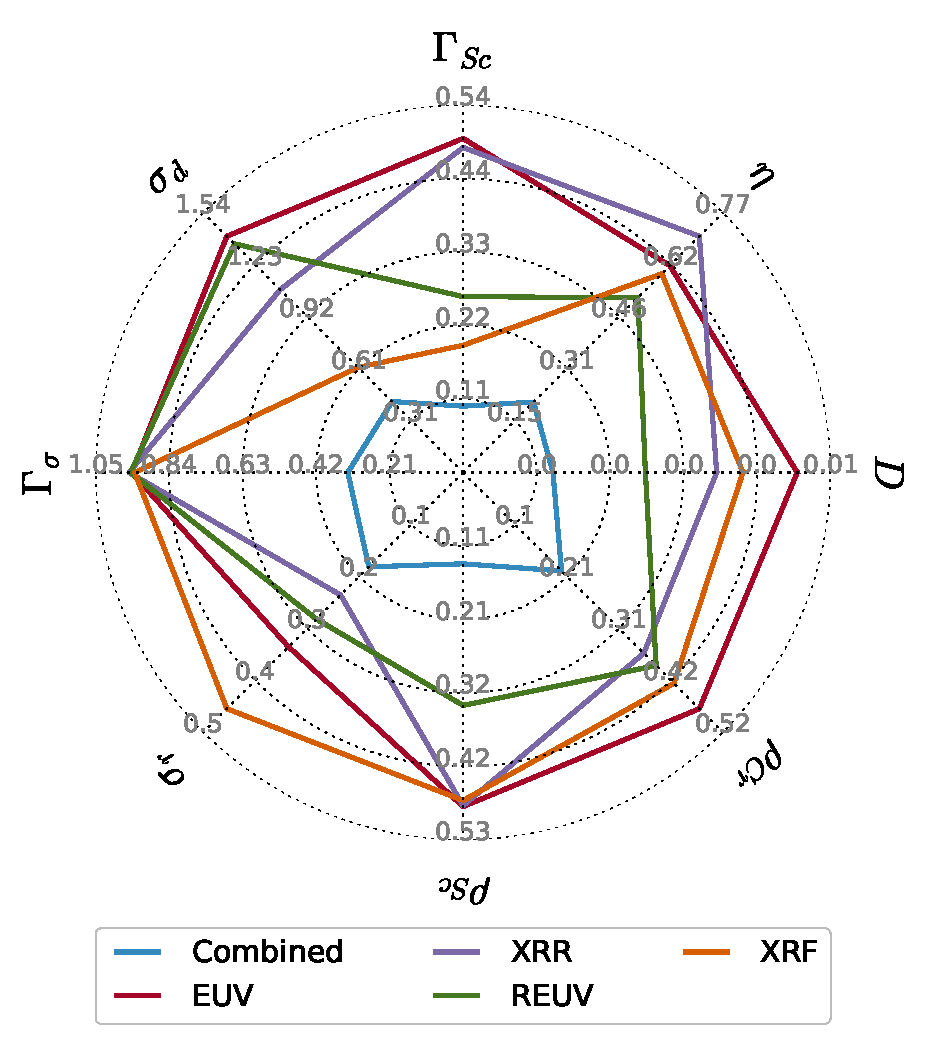
\includegraphics[width=0.6\textwidth]{img/im_cr_sc_multilayer/spiderplot_confidence_intervals_empty}
  \caption{Visualization of the total confidence intervals for each of the parameters with respect to each of the individual experiments as well as the combined analysis.}
  \label{fig:confidence_intervals}
\end{figure}
It is worth noting that the confidence interval for the combined analysis is significantly smaller compared to the individual experiments. This is especially true for the parameter $\Gamma_\sigma$ describing the asymmetry of the interdiffusion layers. Within each of the individual experiments this parameter remains undefined, while the combined analysis delivers significant result of clearly asymmetric interdiffusion layer thicknesses.


\section{Results and Discussion}

The best fit result based on the two-step optimization procedure of the combined data set of all experiments are shown in Fig.~\ref{fig:combined_fit_result} together with the experimental data. The theoretical calculations based on the above model and the experimental data show a good agreement. Nevertheless, differences can be observed. The reason lies in the fact that each experiment was conducted in different experimental setups. Additionally, the beam divergence could not be considered in the analysis of the XRF experiment leading to less pronounced curve shapes in the experimental data than in the theoretical calculations. These deviations affect the confidence intervals given in Table~\ref{tbl:results} and are therefore taken into account. They lead to an increase the uncertainty of the end result.
\todo{Maybe it is possible to give uncertainty values for the best case? perfect homogeneous sample?}
\onecolumn
\begin{figure}
  \centering
  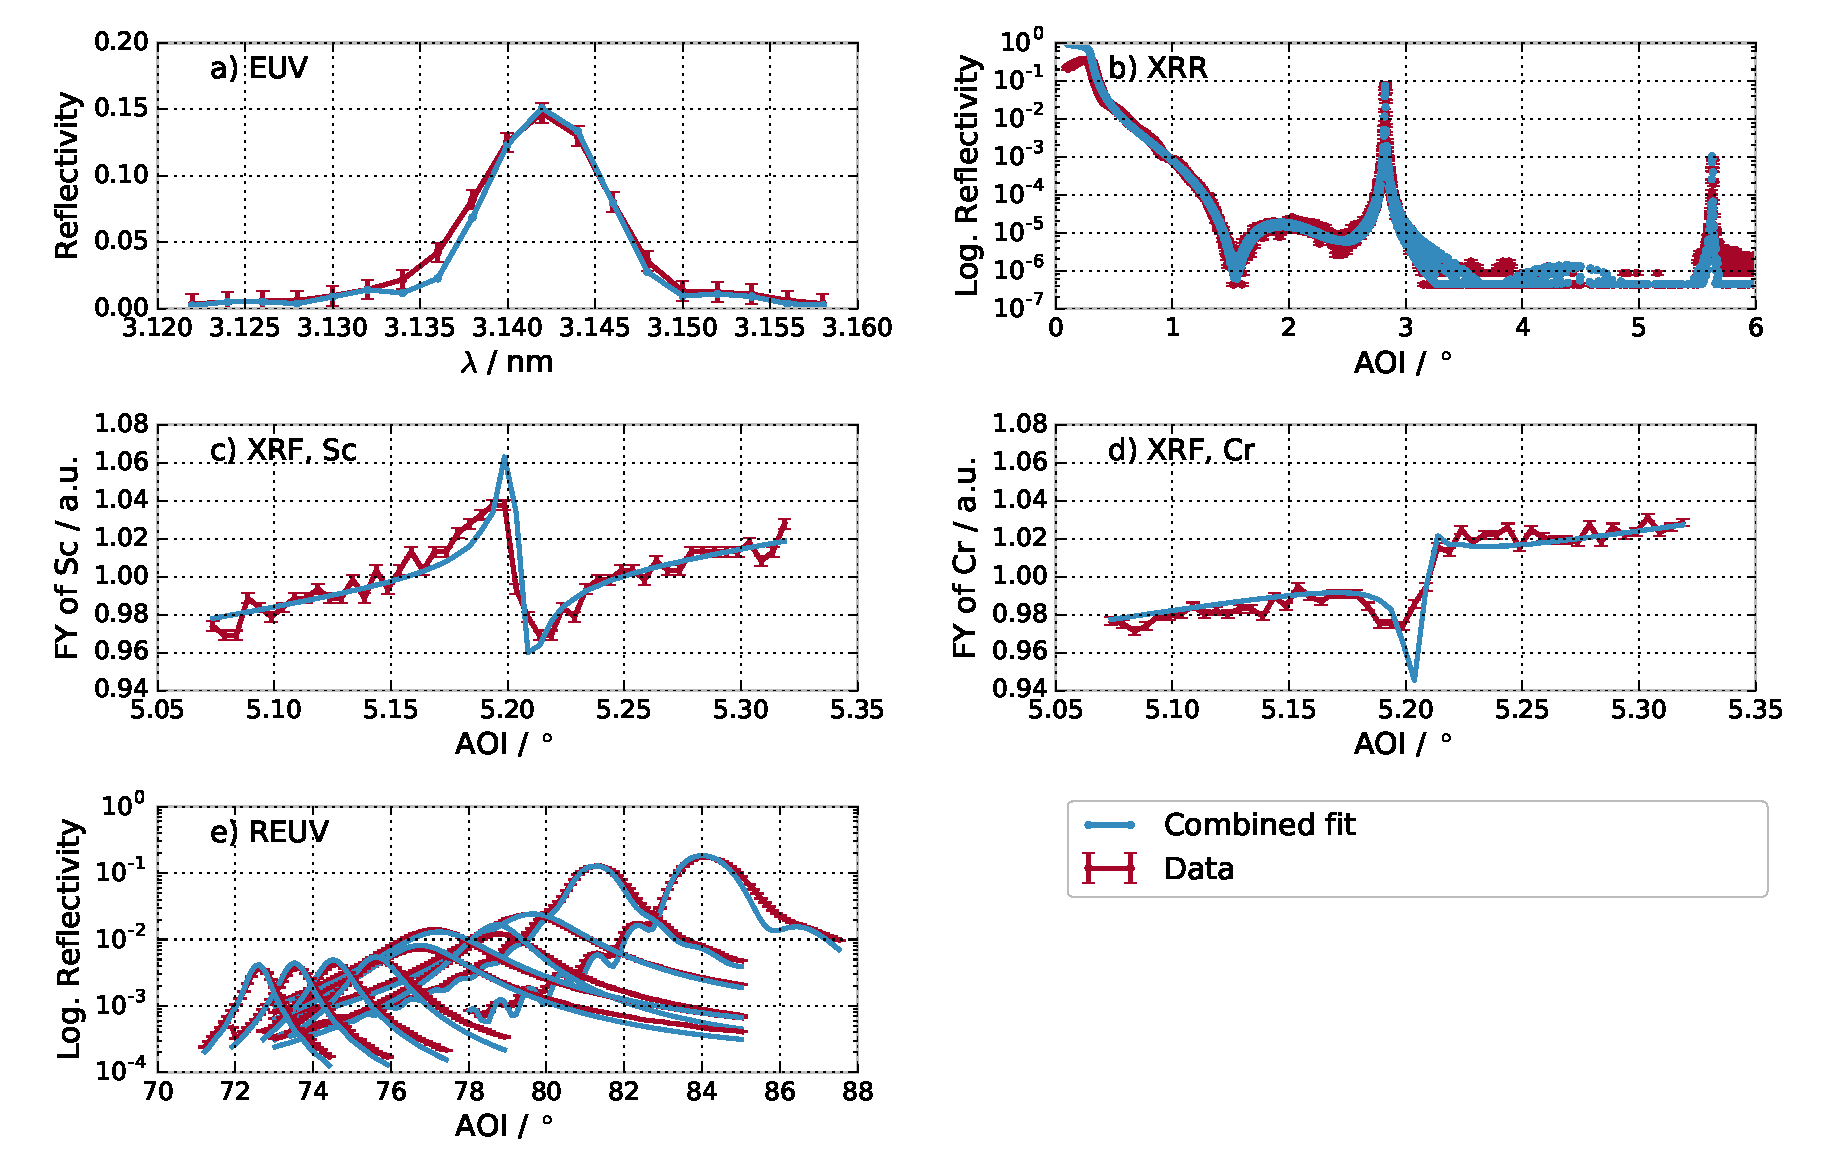
\includegraphics[width=0.9\textwidth]{img/im_cr_sc_multilayer/combined_fit_result}
  \caption{Measured and calculated reflectivity and intensity curves for the optimized parameters with the combined analysis of all experiments as listed in Table~\ref{tbl:parametrization}.}
  \label{fig:combined_fit_result}
\end{figure}

The electron density profile, i.e.~the depth dependence of the index of refraction, can now be constructed explicitly by applying the optimal parameters to the model. The result is shown in Fig.~\ref{fig:electron_density_profile} together with the initial binary model for comparison.
\begin{figure}
  \centering
  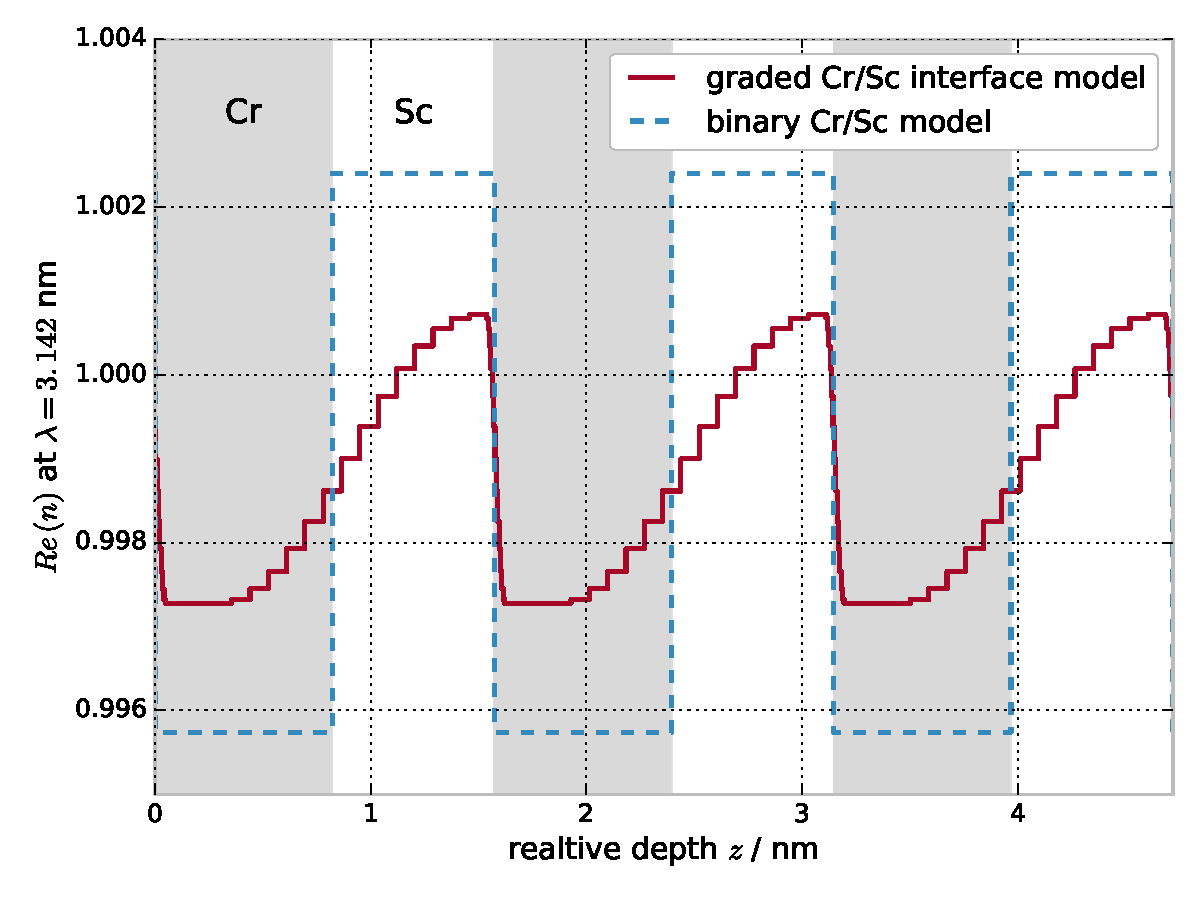
\includegraphics[width=\textwidth]{img/im_cr_sc_multilayer/real_model}
  \caption{Real part of the index of refraction $n$  based on the results of the optimized parameters listed in Table~\ref{tbl:results} for the combined analysis for a selected wavelength. The gradual interface model is shown in direct comparison to the binary model optimized for the EUV reflectivity curve over three full periods. The resulting strong asymmetry in the width of the interface regions is clearly visible (see text). The gray and white shaded areas indicate the Cr and Sc layers, respectively, for the binary model.}
  \label{fig:electron_density_profile}
\end{figure}
An asymmetric distribution of the interdiffusion layers can be observed. This result is only possible due to the combination of all analytic experiments conducted here, as can be seen from the confidence intervals in Fig.~\ref{fig:confidence_intervals} as well as the values in Table~\ref{tbl:results}. A possible physical reason for this effect is the deposition process through magnetron sputtering. The elements Cr and Sc have different mass and thus different momentum when deposited onto each other. A similar effect is known from the deposition of Mo/Si multilayer systems, where the heavier Mo shows higher penetration into the Si layer than vice versa \cite{mosi_asymmetry}. In case of Cr/Sc multilayers, the Cr is heavier and thus has higher momentum leading to a broader interdiffusion layer.
The validation using the MCMC procedure also yield possible correlations between single parameters of the model. In case of the data, methods and model presented here even the combined analysis leaves a correlation between the intermixing parameter $\eta$ and the roughness $\sigma_r$. This means that none of the methods, not even the combined analysis contains sufficient information to deduct a unambiguous result for the roughness or intermixing. Intermixing alone merely reduces optical contrast, while interface roughness causes diffuse scattering. A natural tool for distinguishing between the two is thus provided through the measurement of the diffuse scattering. The distribution of the off-specular scattering with respect to the angle and wavelength provide additional information on the vertical and lateral correlation of spacial roughness frequencies. The latter is described by the power spectral density. We conducted a diffuse scattering experiment as described in Sec.~\ref{sec:experimental}. The 
analysis was done based on the DWBA formalism outlined in Sec.~\ref{sec:matrix_formalism}. The left-hand side of Fig.~\ref{fig:diffuse_meas} shows the measured reciprocal space map in direct comparison to the best-model found within the DWBA approach. The formation of a narrow Bragg sheet \cite{Haase:14,PhysRevLett.73.2228} confirms the high degree of roughness correlation and thereby justifies the approximations made in Sec.~\ref{sec:matrix_formalism} for identical roughness properties at each interface. To deduct the effective power spectral density shown on the right hand side of Fig.~\ref{fig:diffuse_meas} we have taken a cut along the Bragg sheet as indicated by the dashed white lines in the reciprocal space maps and divided it by the multilayer enhancement factor in Eq.~\ref{eqn:dwba} leaving the contribution of the effective PSD $C(q_x)$ to the diffuse scattering.
\onecolumn
\begin{figure}
  \centering
  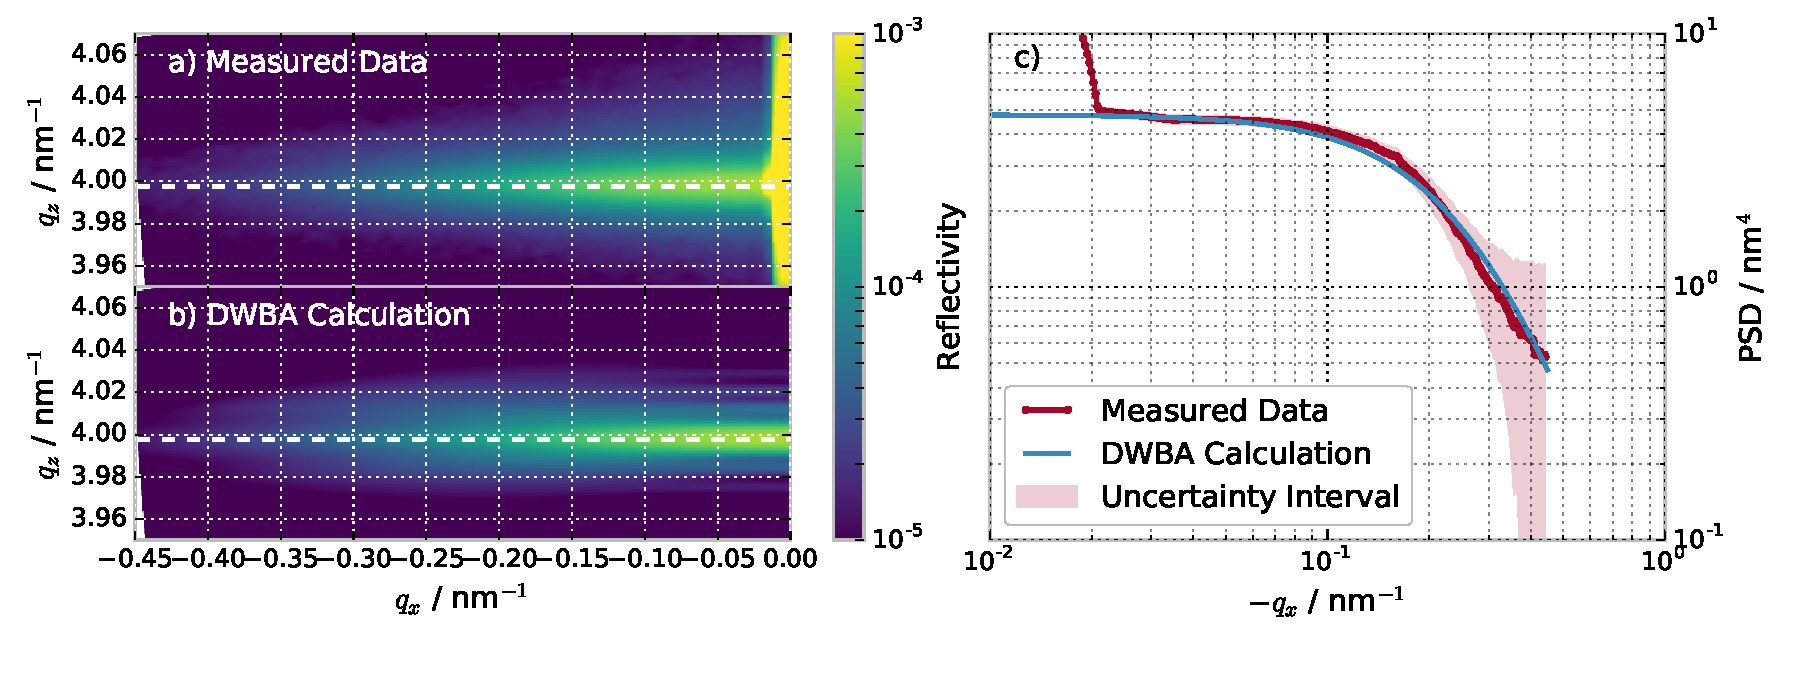
\includegraphics[width=\textwidth]{img/im_cr_sc_multilayer/diffuse_incl_psd}
  \caption{a) Diffuse scattering measurement in $q$-space representation and log scale. b) DWBA Calculation of the optimal PSD model based on the electron density profile with the multilayer parameters for the combined analysis listed in Table~\ref{tbl:results}. c) Comparison of the extracted effective PSDs from the diffuse scattering measurement shown in (a) and the calculation of (b) at the horizontal cut positions indicated by the white dashed lines. The uncertainty interval for the extracted measured data is also indicated.}
  \label{fig:diffuse_meas}
\end{figure}

The best-model results for the vertical replication factor and the power spectral density are given in Table.~\ref{tbl:psd_results}.

\begin{table}
\centering
\caption{Intervals of the parameters entering the PSO procedure}
\label{tbl:psd_results}
\begin{tabular}{@{}ll@{}}
\toprule
Parameter & Best model values\\ \midrule
$\sigma_r$ / nm & $0.187$ \\
$\xi_\parallel$ / nm& $3.3$ \\
$\xi_\perp$  / nm& $7.0$ \\
$H$ & $1.0$ \\
$\beta$ & $0.0$ \\
 \bottomrule
\end{tabular}
\end{table}

\section{Conclusions}

In conclusion we have demonstrated a robust method to characterize ultra-thin multilayer systems with sub-nanometer layer thicknesses unambiguously. Layer thicknesses in the sub-nanometer regime are necessary for near-normal incidence reflective mirrors in the water window spectral range. However, they come with the cost of increasing susceptibility to disturbances of the interfaces at the layer boundaries. This limits the achievable reflectivity to values well below the theoretical threshold posing a demand for ideally non-destructive characterization methods. The main mechanisms diminishing reflectivity are interdiffusion and roughness. With these effects ranging in the order of the layer thickness models based on binary layer stacks become inadequate to describe the physical situation. In order to find a proper representation of the multilayer sample more sophisticated models with explicit description of the gradual interdiffusion layers become necessary. This inevitably increases the numbers of 
parameters of the describing model to be determined in analytical experiments. We performed a rigorous analysis of several analytic methods to determine the model parameters representing the sample. Finding a unambiguous solution is challenging and can only be achieved with a combined analysis of several non-destructive techniques. The optimal set of parameters was determined by applying a particle swarm optimizer in conjunction with a Markov-chain Monte Carlo method to verify the uniqueness of the solution and derive confidence intervals for all parameters in all experiments. The set of analytical methods we employed were EUV and X-ray reflectivity, resonant EUV reflectivity across the Sc L-edge as well as X-ray standing wave fluorescence at the Sc and Cr K-lines across the first Bragg peak. The analysis of each method shows the different sensitivities for specific parameters of the model. The EUV reflectivity shows sensitivity for the optical contrast, i.e. the intermixing $\eta$ and the roughness $\sigma_
r$. With the resonant EUV reflectivity this is further improved and additional sensitivity is added with respect to the ratio of Sc and Cr as well as the total period thickness $D$. The XRR measurement on the other hand yields small confidence intervals for the roughness $\sigma_r$ and also the periodicity $D$. Finally, XRF delivers a method to resolve the multilayer structure spacially and thus the interdiffusion layer thickness $\sigma_d$ and the Sc to Cr ratio. With the combination of all these methods a robust result could be derived with small confidence intervals. Most notably, only the combined analysis can detect the asymmetry of the interdiffusion layers $\Gamma_\sigma$.

Within the small confidence intervals the MCMC methods yields only a single remaining correlation of the intermixing parameter and the roughness factor, which could not be resolved with the experiments in specular geometry. In addition to the combined analysis we therefore added a measurement of the off-specular diffuse scattering to distinguish between the roughness and the interdiffusion. The results of this analysis reveal a high degree of roughness correlation throughout the multilayer with r.m.s.~values comparable with the best fit obtained in the combined analysis and AFM measurements on the top surface layer (not shown here).

    %\include{pFundamentals}
    %\include{pExperimental}
    %\include{pNanometro}
    %\include{pPolymer}
    %\include{pXrr}
    \ifdraft{}{\pagestyle{thesisINTRO}}
    %\include{pSummary}

    %\ifdraft{}{\pagestyle{thesisINTRO}}
    \printbibliography[heading=bibintoc,title={References}]


\backmatter
    \pagestyle{thesisINTRO}
    \pagestyle{empty}
\selectlanguage{ngerman}
\noindent
\section*{Acknowledgement}
At this point, I would like to express my gratitude to all of those who directly or indirectly contributed to the successful completion of this thesis.

First and foremost, I would like to thank Dr.~Frank Scholze, head of the EUV radiometry group at the Physikalisch-Technische Bundesanstalt, for giving me the chance to conduct the work leading to this PhD thesis under his supervision. Our numerous scientific discussions, his valuable ideas and his constructive criticism bundled with the opportunity to conduct experiments even on a short notice, contributed significantly to the success of this thesis.

Furthermore, I would like to thank Prof.~Dr.~Mathias Richter for his support and the examination of this thesis. He always had an open ear and valuable advise for the course of my scientific work and the near future. 

I am very grateful to Prof.~Dr.~Stefan Eisebitt for supporting and evaluating my dissertation and to Dr.~Sa\v{s}a Bajt for the fruitful discussions and collaboration, for providing me with the Cr/Sc samples for my experiments and her willingness to serve as evaluator of this thesis. In addition, I thank Dr.~Stefan Braun for contributing the Mo/Si multilayer mirror samples.

I also like to acknowledge all of my current and former colleagues and fellow graduate students, first of all my mentor, Dr.~Victor Soltwisch, who supported me during the past years. I would also like to thank Anal\'{i}a Fern\'{a}ndez Herrero, Raül Garc\'{i}a Diez, Dr.~Christian Gollwitzer, Dr.~Philipp Hönicke, Mika Pflüger and Dr.~Jan Wernecke. Our many intense discussions and the collaborative atmosphere they helped to establish improved my research significantly.

I am sincerely grateful to all members of the working group 7.12, Christian Buchholz, Ayhan Babalik, Anja Babuschkin, Martin Biel, Benjamin Dubrau, Andreas Fischer, Anne Hesse, Sina Jaroslawzew, Florian Knorr, Dr.~Christian Laubis, Jana Lehnert, Heiko Mentzel, Jana Puls, Anja Schönstedt, Christian Stadelhoff. Without their support and patience in many late-night beamtimes in the laboratory, this work would not have been possible. My honest thanks also go to all other colleagues of the PTB in Berlin-Adlershof.

Finally, I am in dept to all of my friends and family for their endless support and their distractions during my studies and over the course of my PhD thesis. Most importantly I would like to name Michl, Michael, Paul, Laura, Tim, Anna, Leo and my parents Detlev and Martina. Last but not least, I am deeply grateful to my grandfather Dr.~Walther Neudert for inspiring me and his early encouragement of my scientific career.








\cleardoublepage

    \selectlanguage{ngerman}

\section*{Eidesstattliche Versicherung}
\vspace{3ex}

Hiermit versichere ich an Eides statt, dass ich die vorliegende Arbeit selbstständig verfasst und keine anderen als die in der Dissertation angegebenen Quellen und Hilfsmittel benutzt habe.
Alle Ausführungen, die anderen veröffentlichten oder nicht veröffentlichten Schriften wörtlich oder sinngemäß entnommen wurden, habe ich kenntlich gemacht.
Die Darstellung des Eigenanteils an bereits publizierten Inhalten in meiner beigefügten Erklärung ist zutreffend.
\vspace{3cm}

\noindent Berlin, den \today \hfill Anton Haase

\cleardoublepage

    %% publication list
\noindent
\pagestyle{empty}
\selectlanguage{ngerman}

\section*{Erklärung}

Es wurden bereits Teile der Dissertation veröffentlicht.
\vspace{2ex}

Liste der Veröffentlichungen, welche in die Dissertation eingeflossen sind:

\begin{enumerate}[label=\arabic*) ]
    \item \fullcite{haase_role_2014} 

    \item \fullcite{haase_characterization_2015} 

    \item \fullcite{haase_multiparameter_2016} 

    \item \fullcite{haase_interface_2017} 

\end{enumerate}
Liste der Veröffentlichungen, welche nicht in die Dissertation eingeflossen sind:
\begin{enumerate}[label=\arabic*) ]
    \item \fullcite{prasciolu_extended_2015} 

    \item \fullcite{soltwisch_correlated_2016} 
    
\end{enumerate}


Ich habe an keiner anderen Hochschule oder Fakultät eine Promotionsabsicht eingereicht.

\vspace{3cm}

\noindent Berlin, den \today \hfill Anton Haase

\cleardoublepage


    %\ifdraft{}{%
        %\printglossary[title=Glossary]
        %\printglossary[type=\acronymtype,title=Abbreviations,style=list]
        %\printglossary[type=symbols,title=Symbols,style=long,nonumberlist=true]
    %}

\end{document}
